\section{Analysis: Iterative RAG Performance and Behavior Patterns}

\subsection{Introduction to Iterative RAG Advantages}

Our iterative RAG system demonstrates significant performance improvements over traditional full-context (gold) approaches across diverse models and question complexities. Through comprehensive analysis of 1,186 multi-hop scientific questions across six state-of-the-art language models, we uncover three critical insights: (1) iterative retrieval provides substantial accuracy gains compared to gold context, (2) models exhibit distinct behavioral patterns in iterative settings, and (3) specific failure modes reveal opportunities for targeted system improvements.

\subsection{Performance Gains: Iterative RAG vs. Gold Context}

\subsubsection{Overall Performance Improvement}

Our evaluation reveals that iterative RAG consistently outperforms full gold context across all tested models (Figure~\ref{fig:correctness_by_steps}). Using the re-verification summary (src/results/reverify_accuracies.csv), accuracy improvements span \textbf{+2.7 to +25.6 percentage points} over gold-context baselines, with a \textbf{median improvement of ~+11.3 pp}. This counterintuitive result---where iteratively retrieved context outperforms complete gold standard context---suggests that strategic, focused information delivery is more effective than overwhelming models with comprehensive documentation.

\paragraph{Key Performance Metrics (Iterative RAG vs. Gold Context):}
\begin{itemize}
    \item \textbf{GPT-5}: 80.9\% vs. 71.7\% \;(\(~\!+9.2\) pp)\footnote{Gold-context baseline for GPT-5 is 0.7168, consistent with analysis scripts.}
    \item \textbf{GPT-4o}: 82.0\% vs. 56.3\% \;(\(~\!+25.6\) pp)
    \item \textbf{Claude 3.7 Sonnet}: 84.5\% vs. 68.1\% \;(\(~\!+16.4\) pp)
    \item \textbf{Claude 3.7 Sonnet + Reasoning}: 86.1\% vs. 73.3\% \;(\(~\!+12.8\) pp)
    \item \textbf{DeepSeek R1}: 82.3\% vs. 72.5\% \;(\(~\!+9.8\) pp)
    \item \textbf{Mistral Large}: 75.3\% vs. 72.6\% \;(\(~\!+2.7\) pp)
\end{itemize}

The performance advantage is especially evident on questions where evidence curation matters most, consistent with an iterative process that filters, stages, and focuses evidence over steps rather than presenting raw, exhaustive context all at once.

\begin{figure}[t]
    \centering
    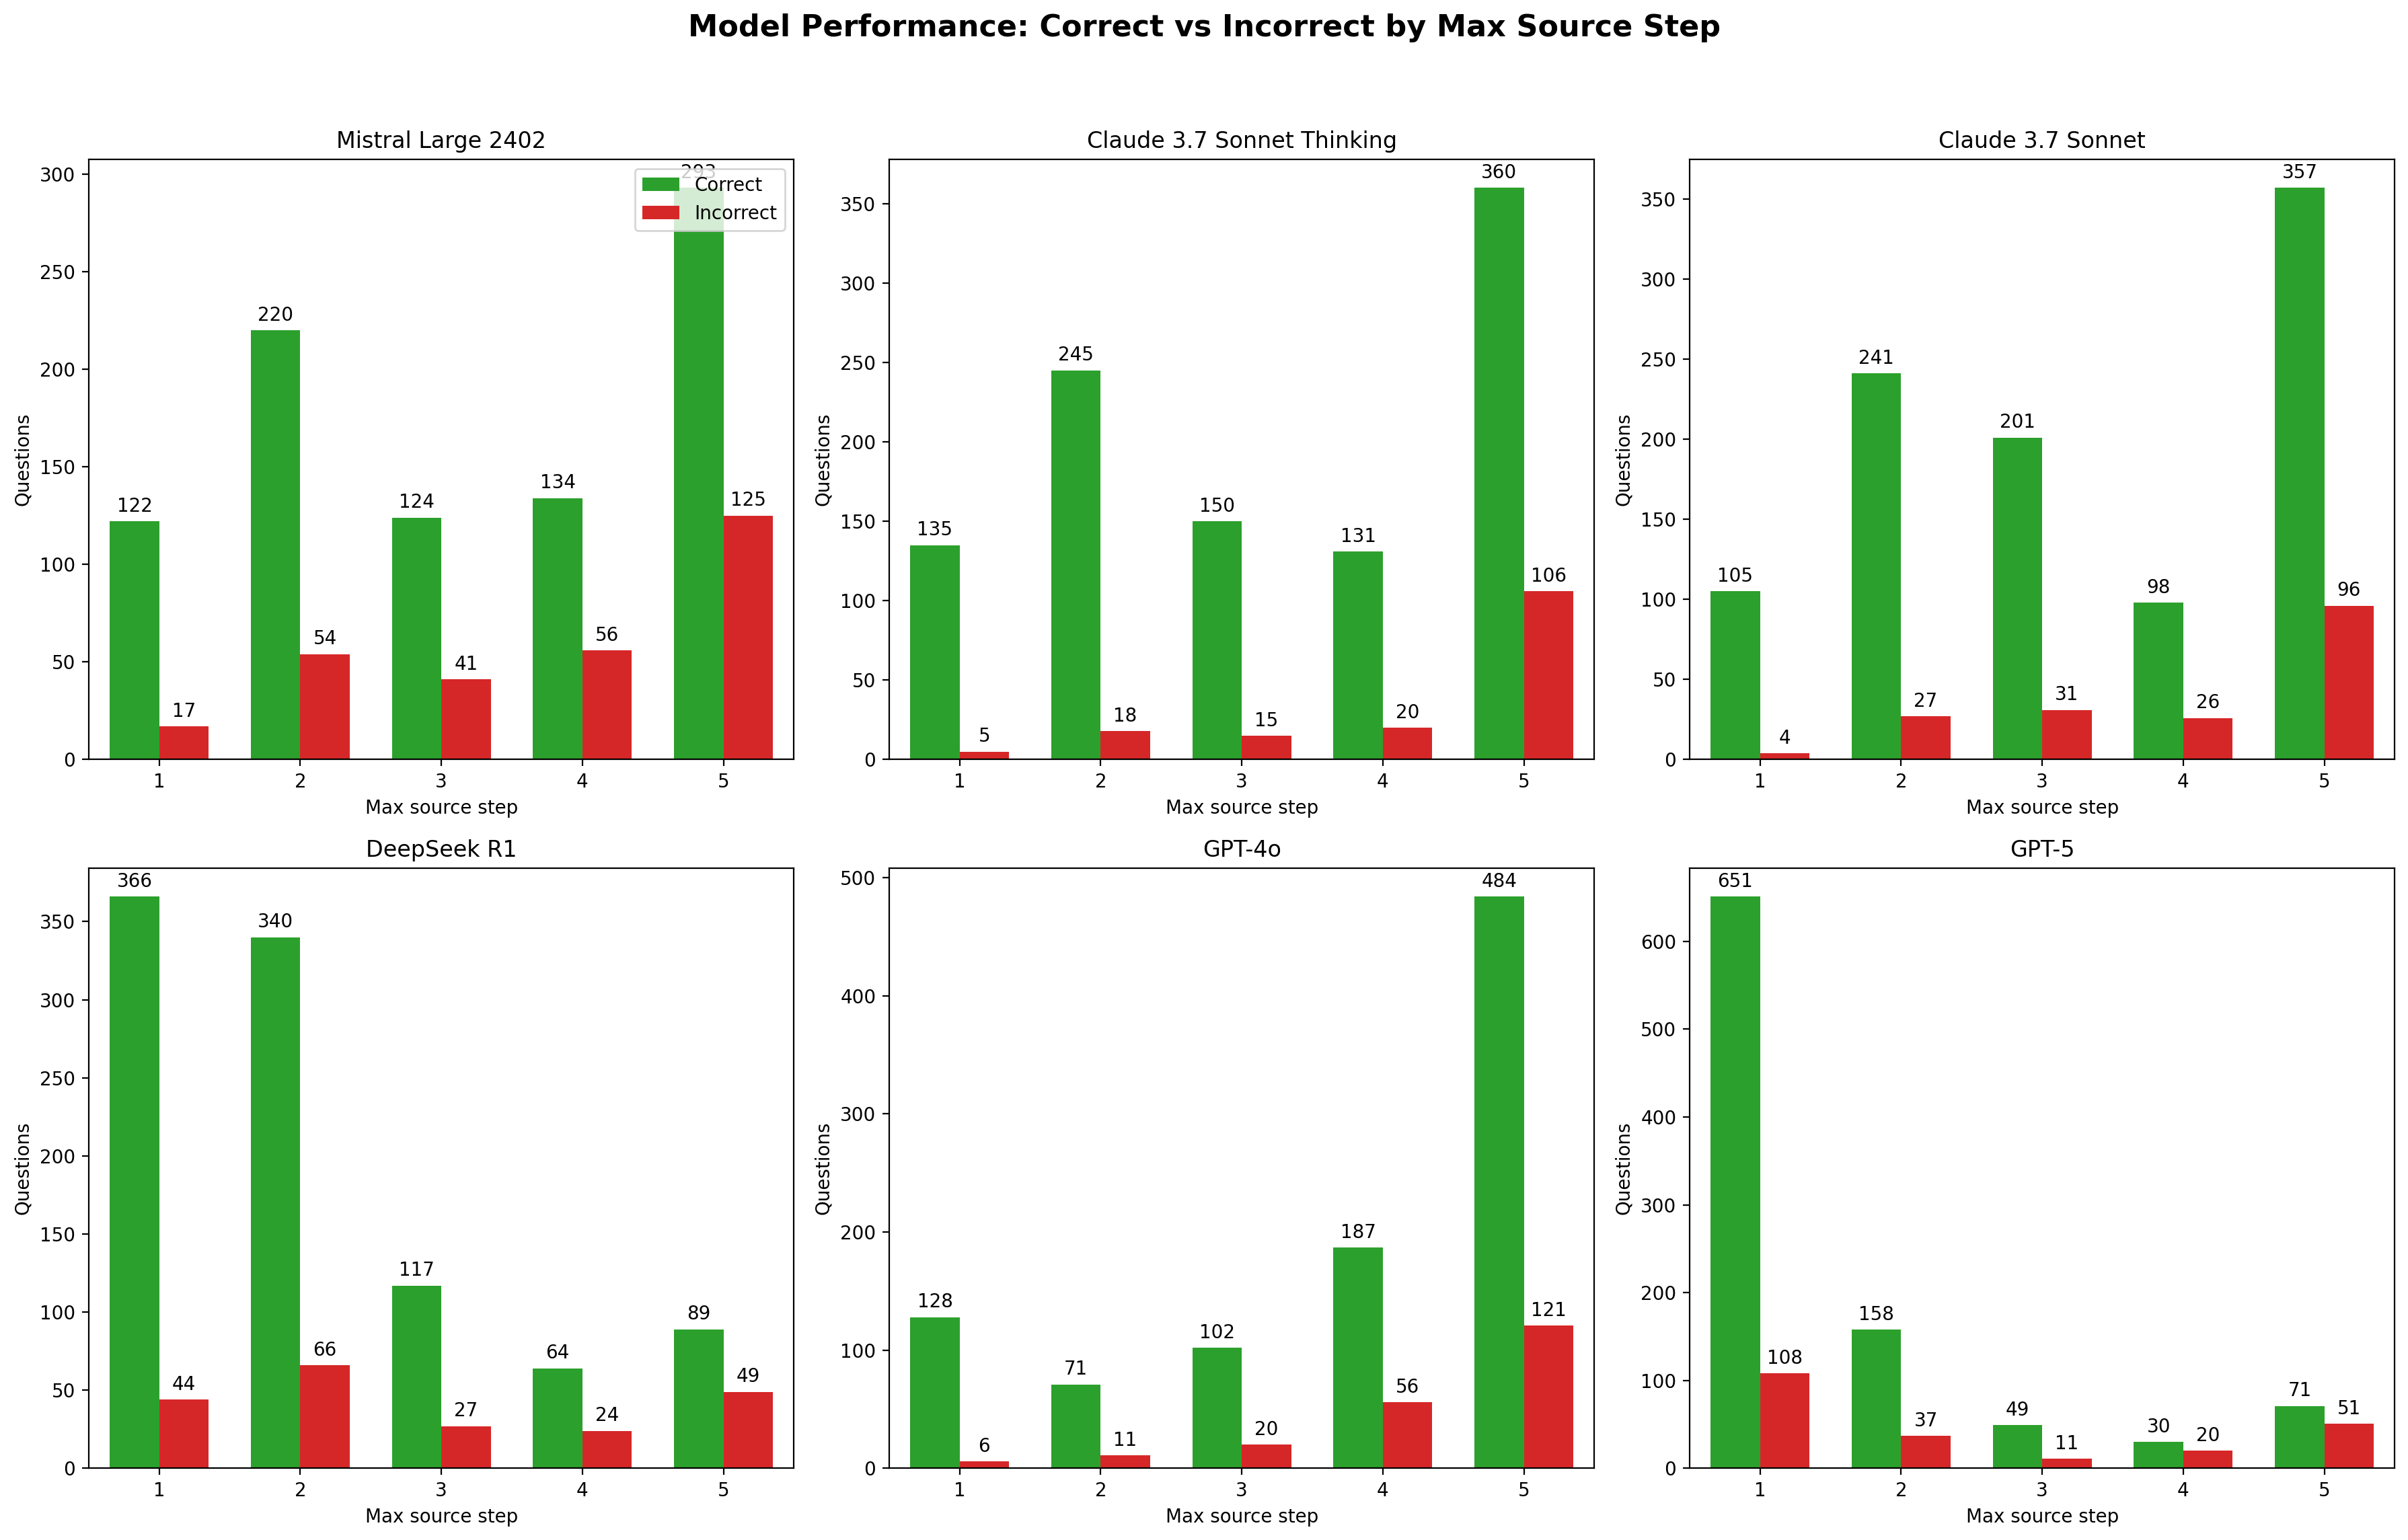
\includegraphics[width=0.9\linewidth]{src/chosen_plots/all_models_correctness_by_steps.png}
    \caption{Step-by-step correctness progression across all models, showing rapid accuracy gains in early steps (1--3) with diminishing returns after step 4.}
    \label{fig:correctness_by_steps}
\end{figure}

\subsubsection{Step-by-Step Accuracy Progression}

Analysis of correctness by retrieval steps (Figure~\ref{fig:correctness_by_steps}) reveals a characteristic progression pattern. Models typically realize most of their gains in the early steps (1--3), with diminishing returns thereafter. This indicates that additional retrieval iterations are valuable when they improve evidence quality, but not when they simply extend the step count.

Notably, question difficulty significantly impacts the optimal number of retrieval steps:
\begin{itemize}
    \item \textbf{Simple questions (1--2 hops)}: Converge by step 2--3
    \item \textbf{Medium complexity (3 hops)}: Optimal at step 3--4
    \item \textbf{High complexity (4+ hops)}: Require 4--6 steps but show higher variance
\end{itemize}

This step-wise analysis indicates that adaptive stopping strategies could improve efficiency without sacrificing accuracy---a key insight for practical deployment.

\subsubsection{Unanswered Question Reduction}

The iterative approach reduces unanswered questions compared to single-pass retrieval (Figure~\ref{fig:unanswered_counts}). We observe consistent drops across models, consistent with the loop’s ability to reformulate queries and explore alternative evidence paths when the first attempts fall short.

\begin{figure}[t]
    \centering
    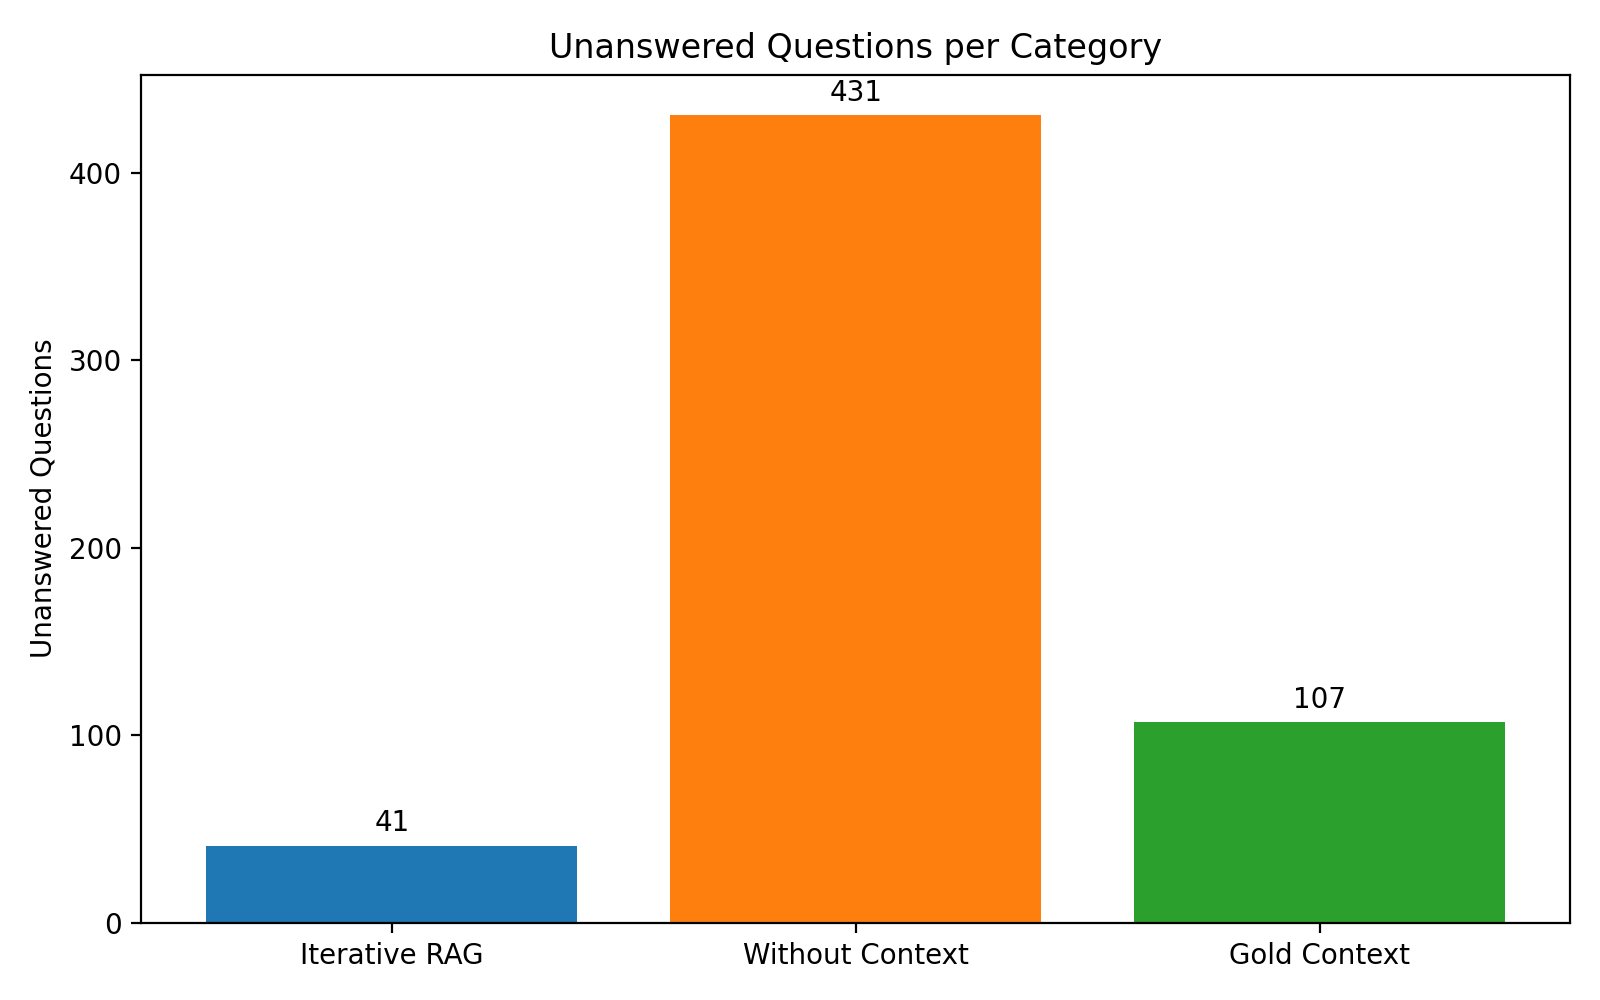
\includegraphics[width=0.7\linewidth]{src/chosen_plots/unanswered_counts.png}
    \caption{Unanswered question counts by model. Iterative retrieval reduces unanswered questions relative to single-pass approaches.}
    \label{fig:unanswered_counts}
\end{figure}

\subsection{Model-Specific Behavioral Patterns}

\subsubsection{Reasoning Token Utilization}

Analysis of reasoning and output token consumption reveals distinct model strategies (Figure~\ref{fig:token_usage}). Models exhibit three categories of behavior:

\paragraph{Category 1: Efficient Reasoners (GPT-4o, GPT-5)}
\begin{itemize}
    \item Maintain relatively consistent token usage across steps
    \item Show minimal increase in reasoning overhead with question complexity
    \item Achieve high accuracy with lower computational cost
\end{itemize}

\paragraph{Category 2: Extended Reasoners (Claude 3.7 + Reasoning, DeepSeek R1)}
\begin{itemize}
    \item Utilize higher token budgets with explicit reasoning traces
    \item Reasoning token usage often increases with question complexity
    \item Higher computational cost but improved performance on complex questions
\end{itemize}

\paragraph{Category 3: Variable Reasoners (Claude 3.7 Sonnet, Mistral Large)}
\begin{itemize}
    \item Token usage varies significantly by question type
    \item Less consistent reasoning patterns
    \item Moderate performance with moderate computational requirements
\end{itemize}

Critically, for the hardest questions (4--6 models wrong), \textbf{correct answers use markedly fewer tokens} than incorrect attempts (Figure~\ref{fig:hard_questions_tokens}), indicating that successful reasoning is more concise and focused rather than exhaustive.

\begin{figure}[t]
    \centering
    \begin{subfigure}[b]{0.48\linewidth}
        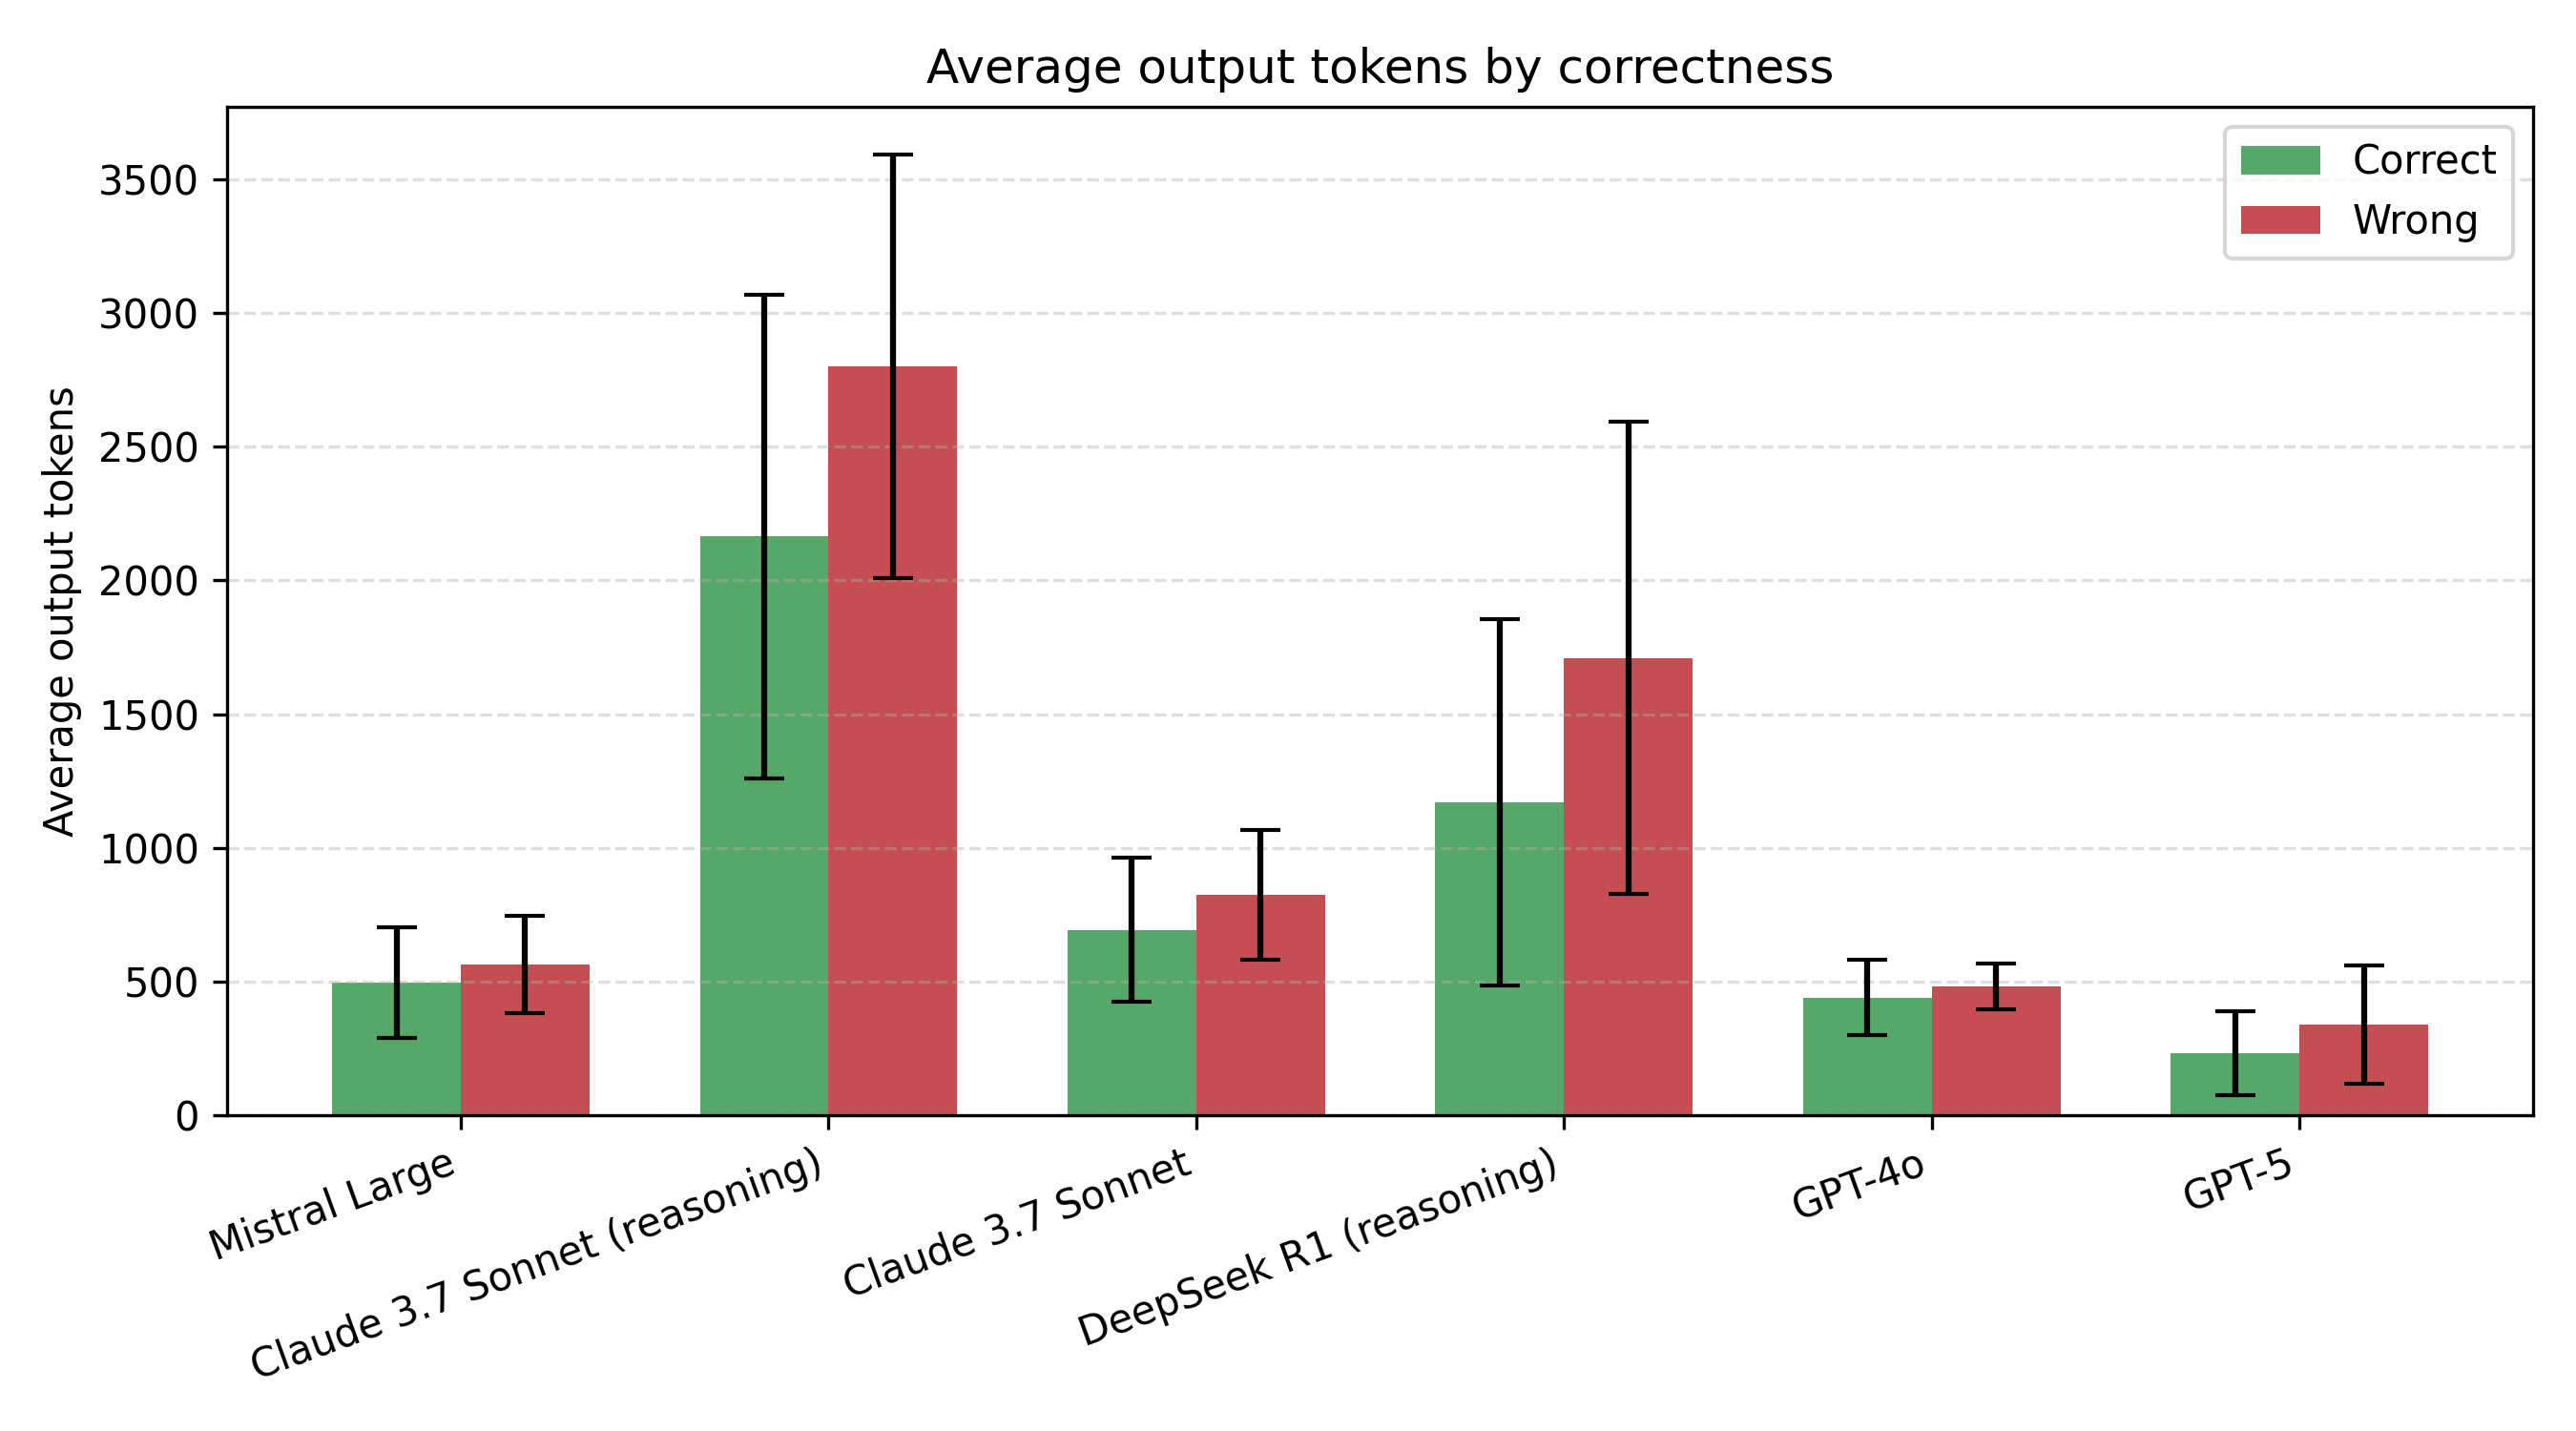
\includegraphics[width=\linewidth]{src/chosen_plots/average_output_tokens.png}
        \caption{Average output tokens}
    \end{subfigure}
    \hfill
    \begin{subfigure}[b]{0.48\linewidth}
        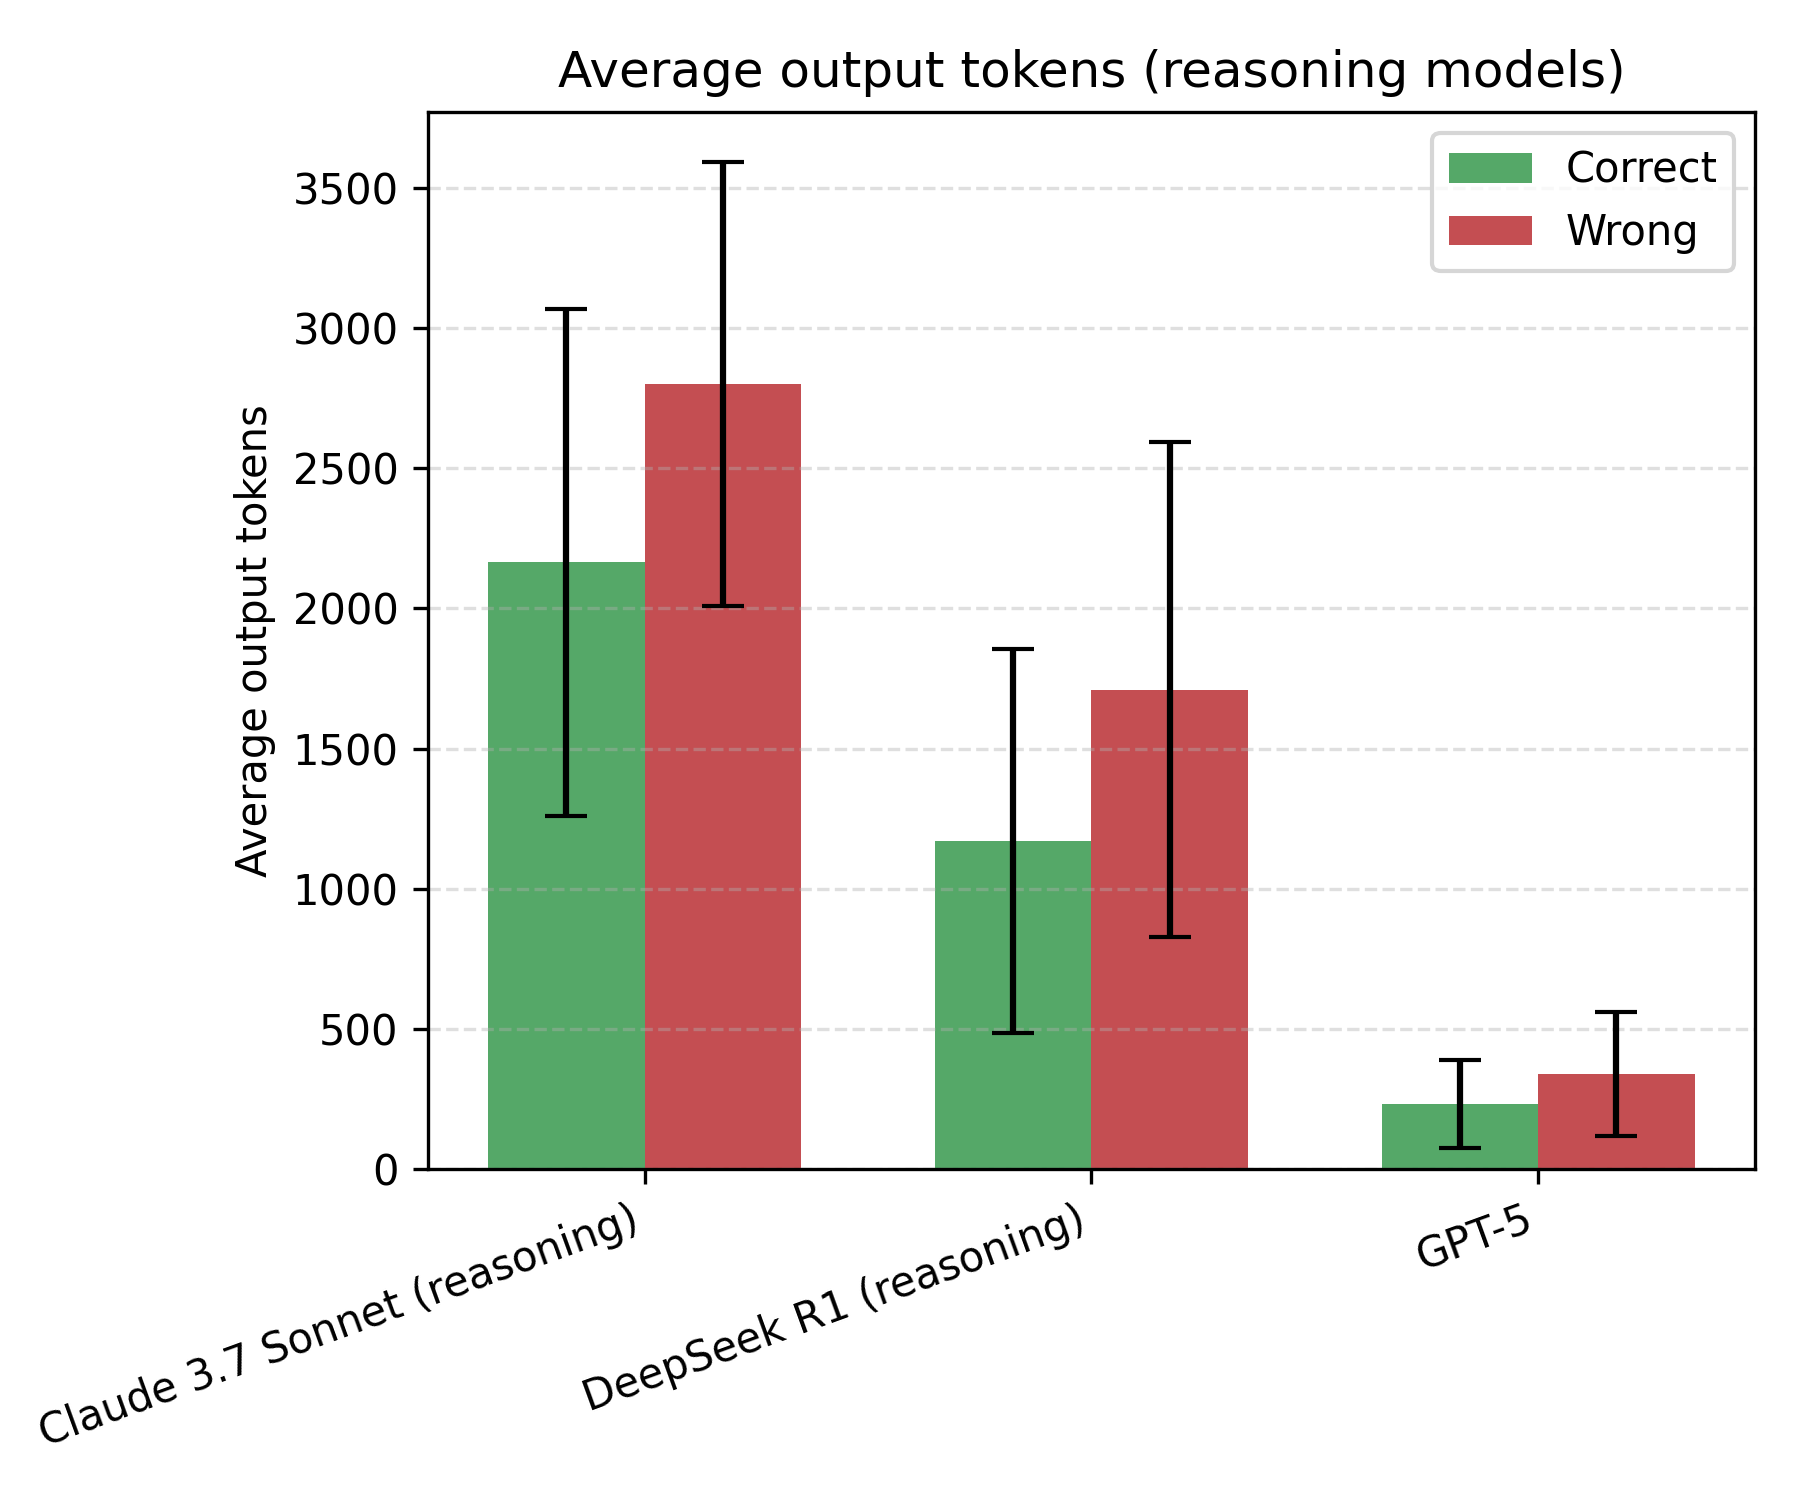
\includegraphics[width=\linewidth]{src/chosen_plots/average_output_tokens_reasoning.png}
        \caption{Reasoning tokens}
    \end{subfigure}
    \caption{Token utilization patterns across models, revealing three distinct reasoning strategies.}
    \label{fig:token_usage}
\end{figure}

\begin{figure}[t]
    \centering
    \begin{subfigure}[b]{0.48\linewidth}
        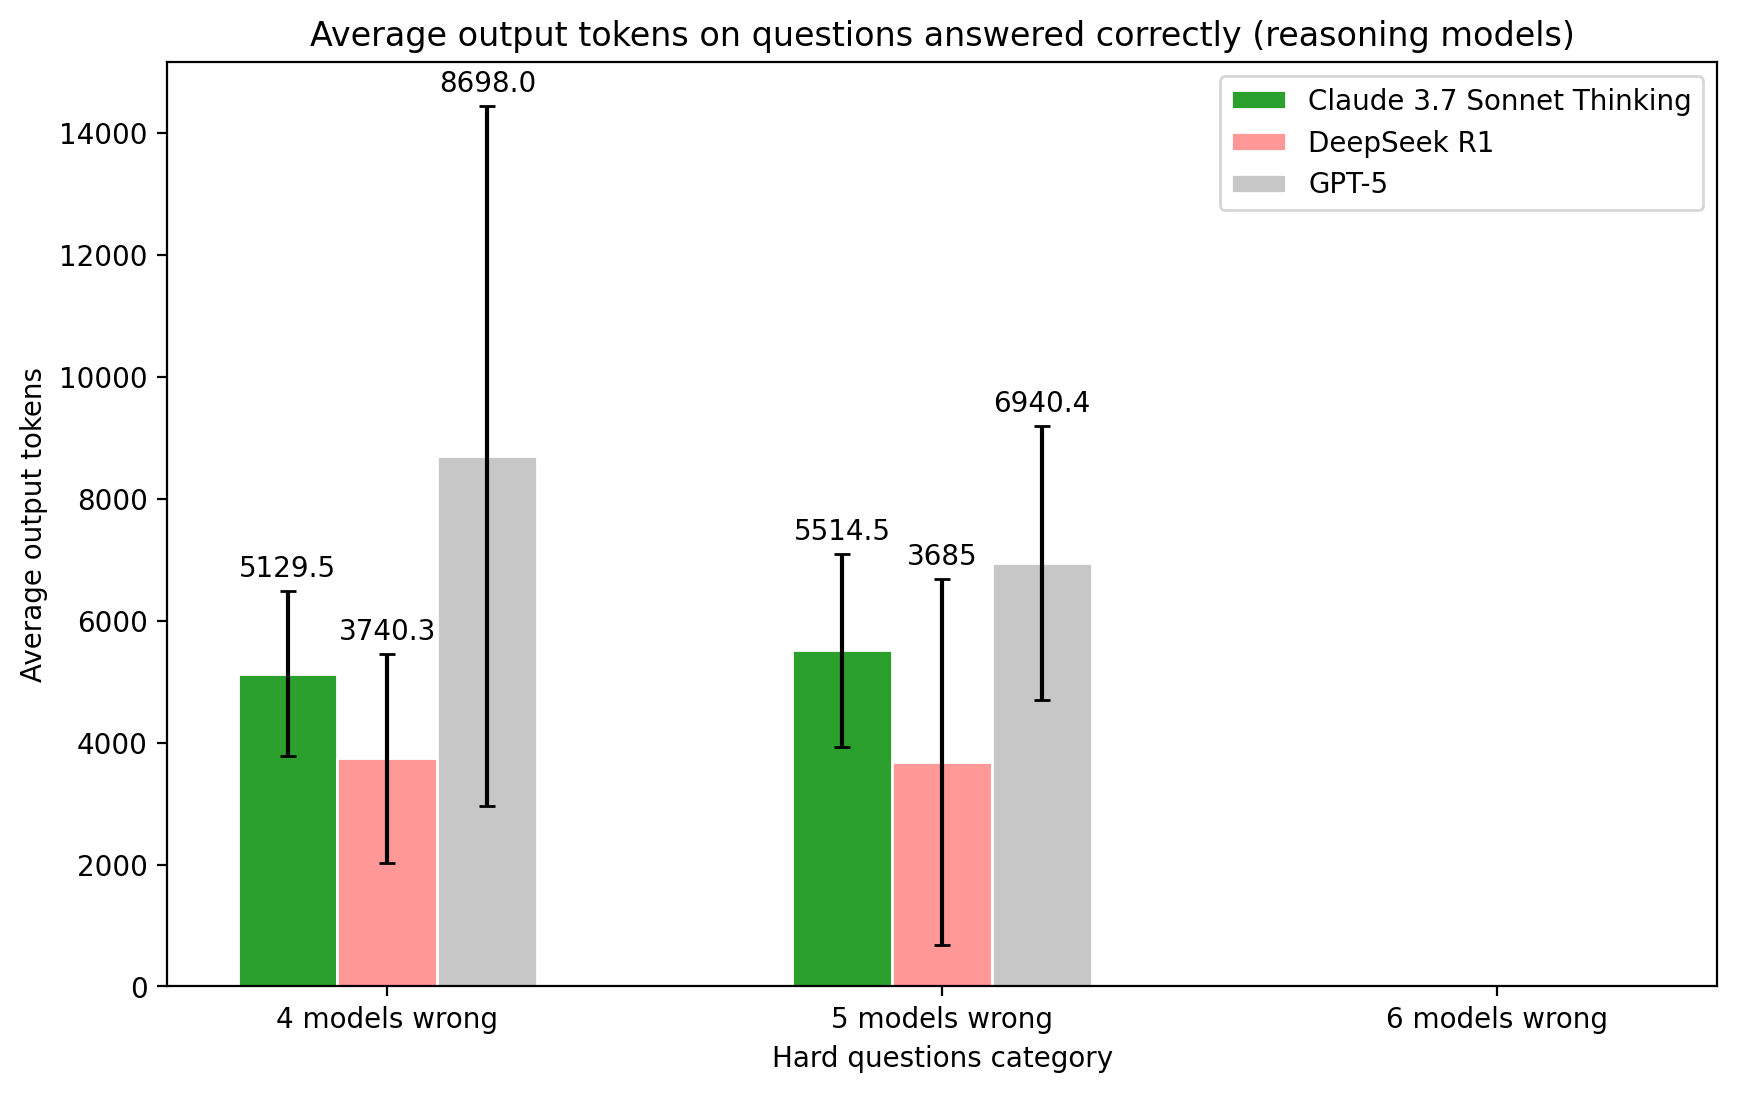
\includegraphics[width=\linewidth]{src/chosen_plots/hard_questions_reasoning_correct_total_tokens.png}
        \caption{Correct answers}
    \end{subfigure}
    \hfill
    \begin{subfigure}[b]{0.48\linewidth}
        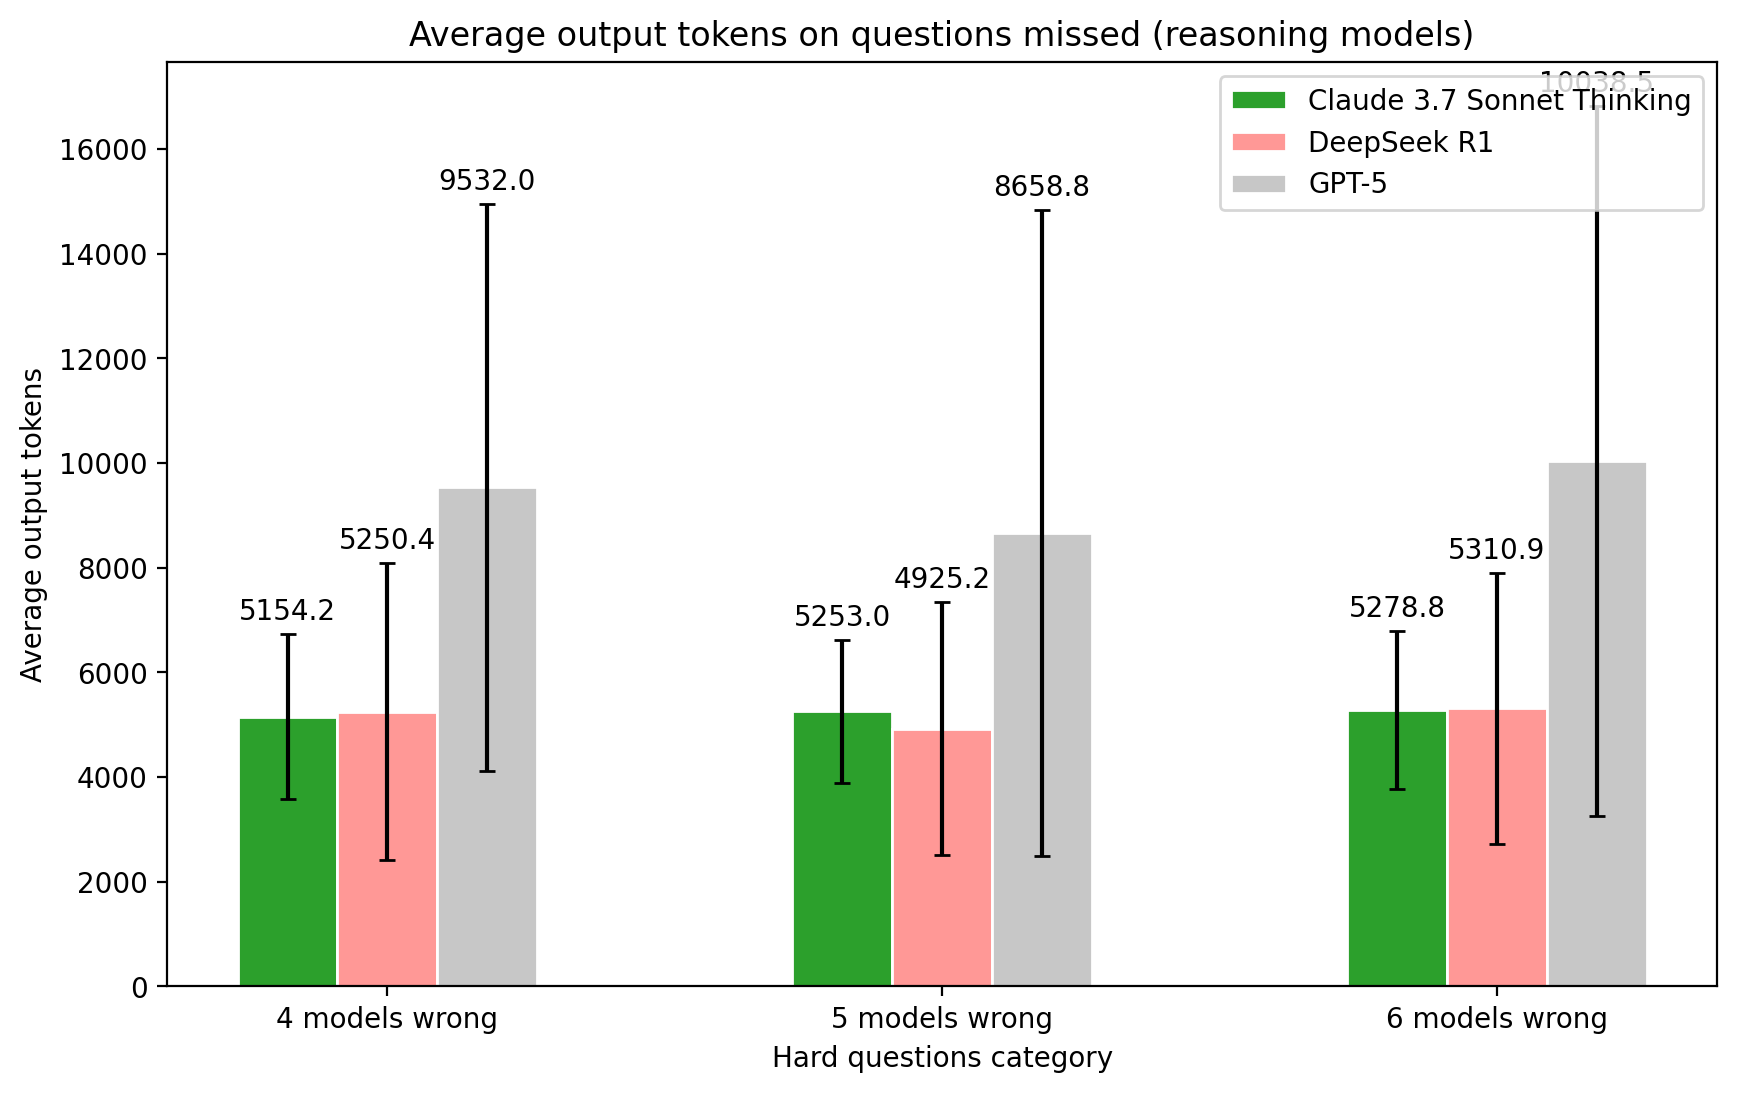
\includegraphics[width=\linewidth]{src/chosen_plots/hard_questions_reasoning_incorrect_total_tokens.png}
        \caption{Incorrect answers}
    \end{subfigure}
    \caption{Token usage on hardest questions (6 models wrong), showing correct answers tend to use substantially fewer tokens than incorrect attempts.}
    \label{fig:hard_questions_tokens}
\end{figure}

\subsubsection{Performance on Hard Questions by Category}

We categorize questions by difficulty based on how many models answer incorrectly (Figure~\ref{fig:hard_questions_categories}). Model behavior diverges sharply on these challenging questions:

\textbf{GPT-5} demonstrates superior robustness on the hardest categories relative to peers, suggesting architectural or training differences that enable better handling of ambiguous or incomplete information.

\textbf{DeepSeek R1} shows high variance---approaching top performance on some types yet collapsing on others---consistent with sensitivity to reasoning trace quality and early query formulation.

\textbf{Claude variants} show consistent difficulty with certain question patterns, particularly those requiring integration of information across 4+ hops. The addition of explicit reasoning improves robustness but does not fully close the gap on the hardest questions.

\begin{figure}[t]
    \centering
    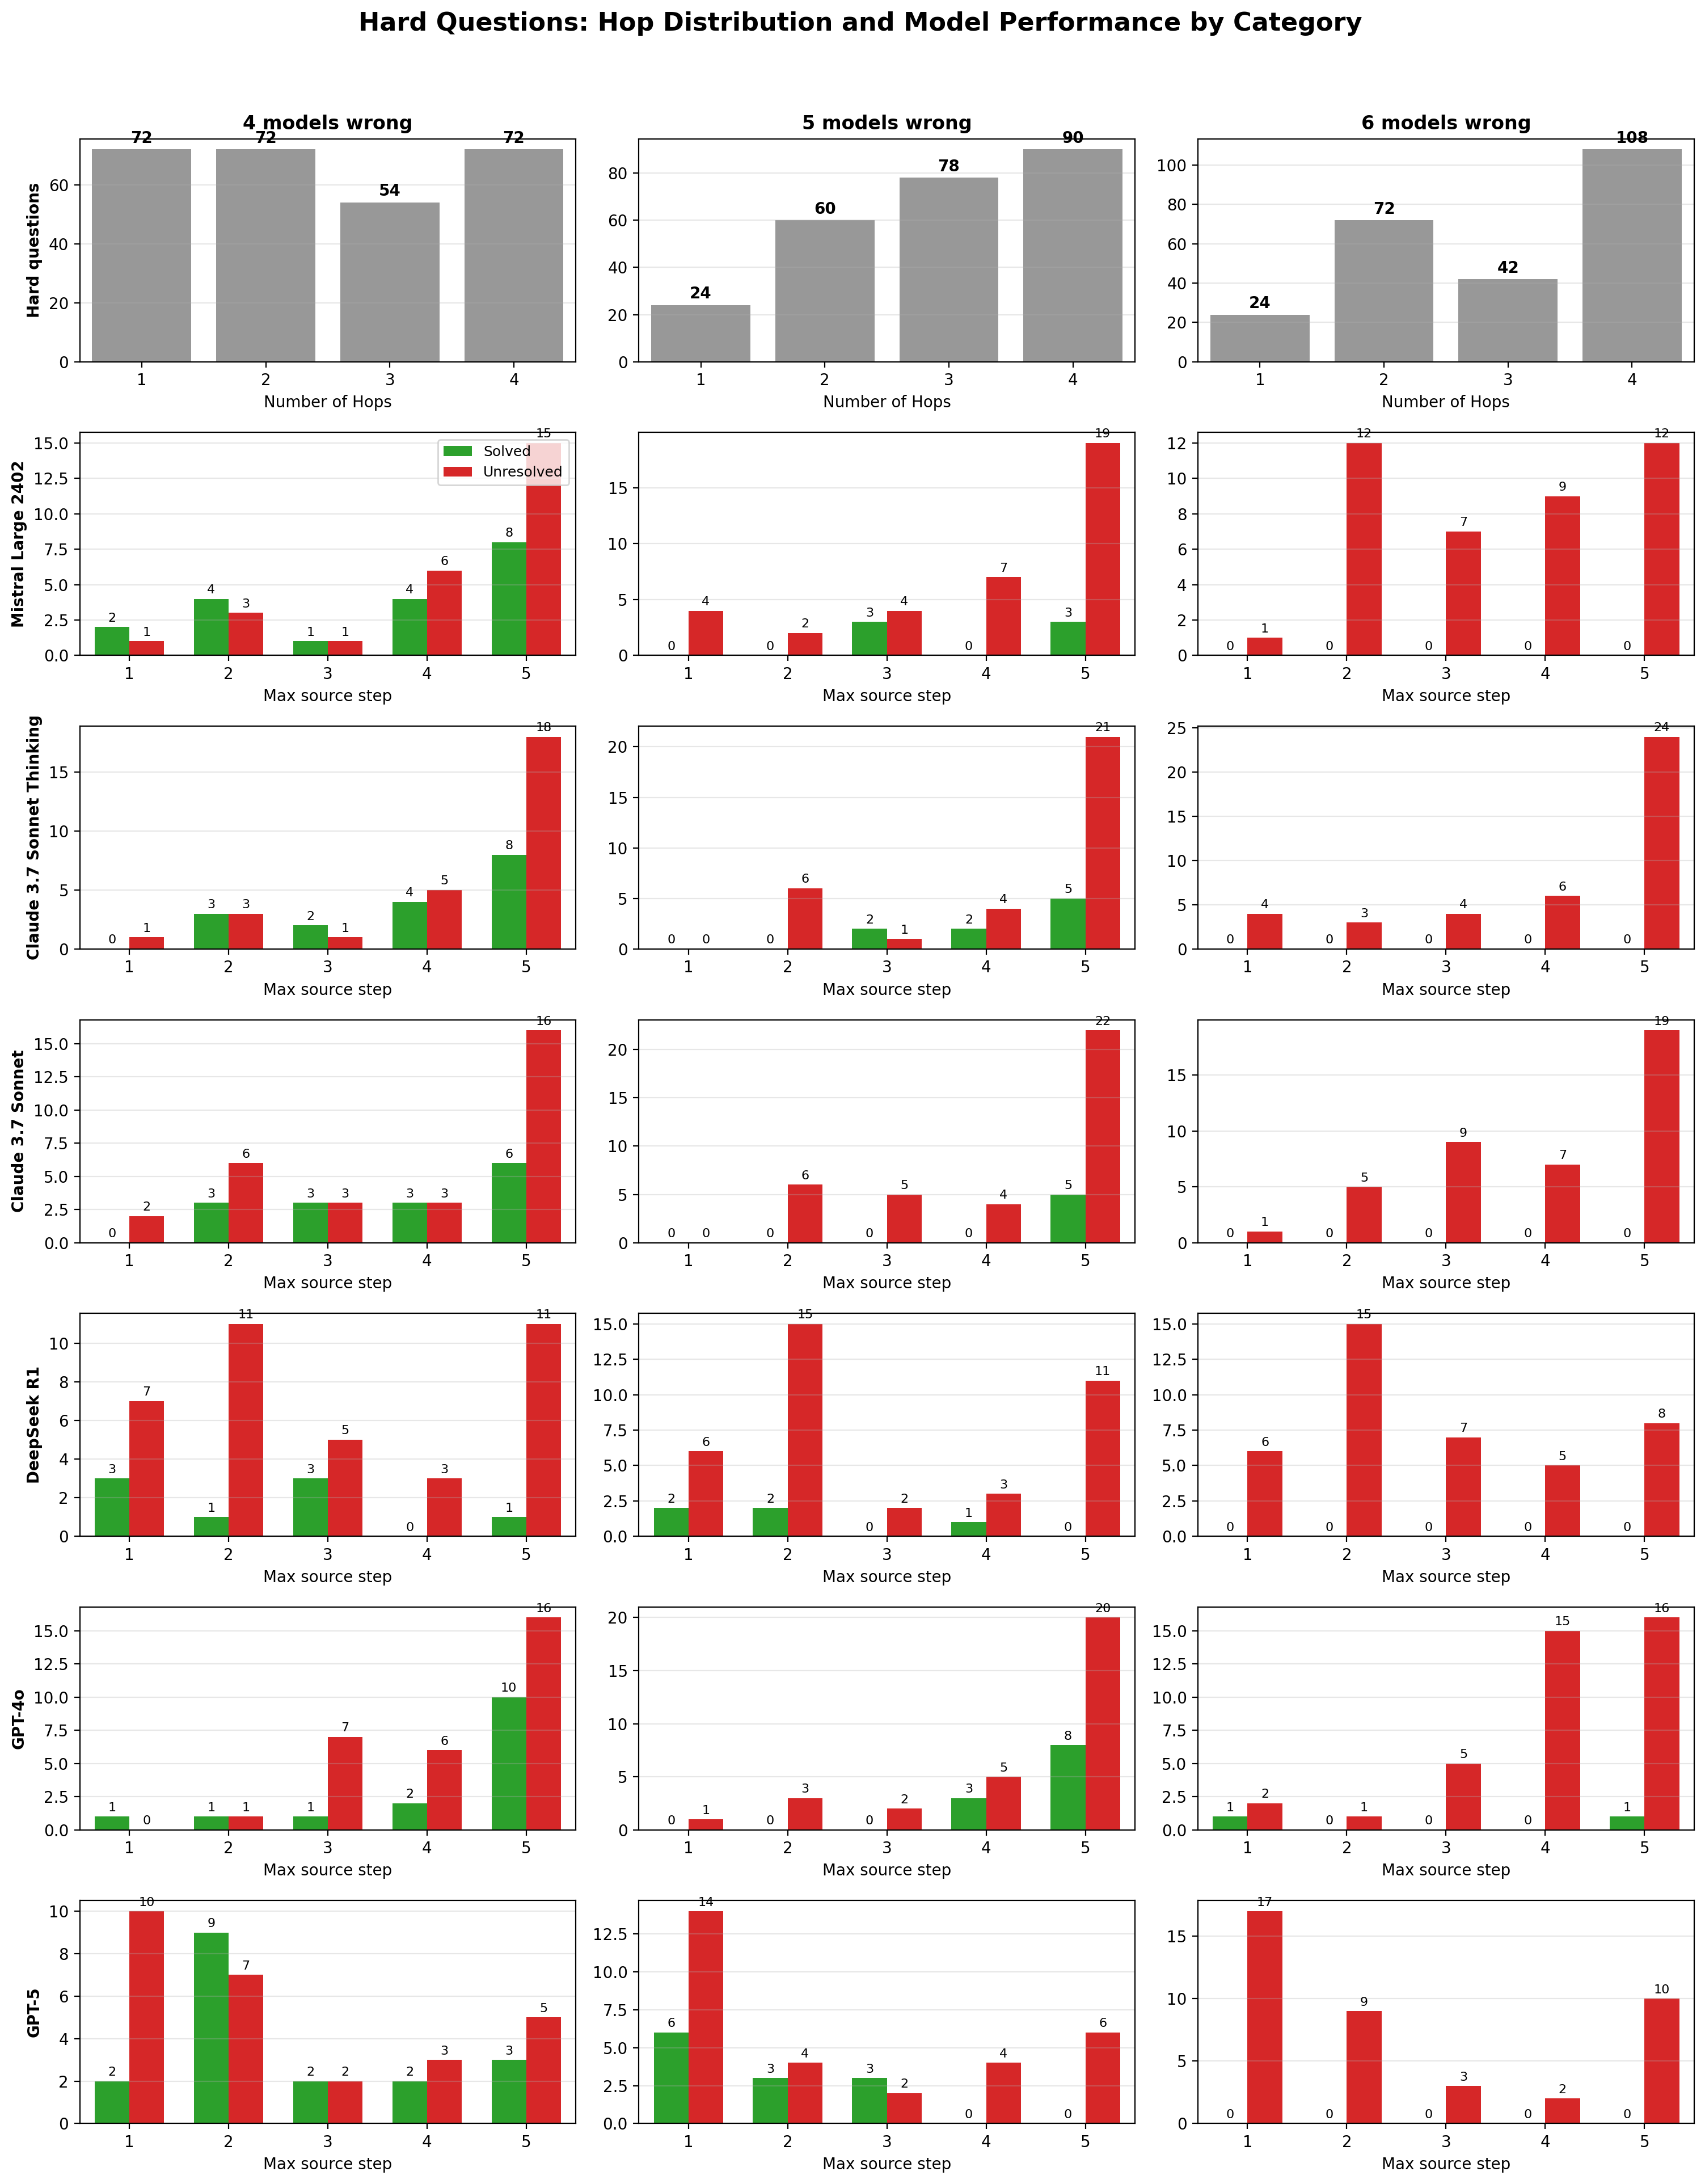
\includegraphics[width=0.95\linewidth]{src/chosen_plots/hard_questions_categories_by_models.png}
    \caption{Hard question performance categorized by difficulty (4/5/6 models wrong), showing model divergence on challenging questions with GPT-5 maintaining robustness while others collapse.}
    \label{fig:hard_questions_categories}
\end{figure}

\subsubsection{Hop Complexity Distribution and Performance}

Question complexity, measured by number of reasoning hops, significantly impacts model performance (Figure~\ref{fig:hop_distributions}). Across models, accuracy declines as hop count increases, and the degradation trends are similar, suggesting a shared structural challenge for multi-hop retrieval and composition rather than purely model-specific weaknesses.

\begin{figure}[t]
    \centering
    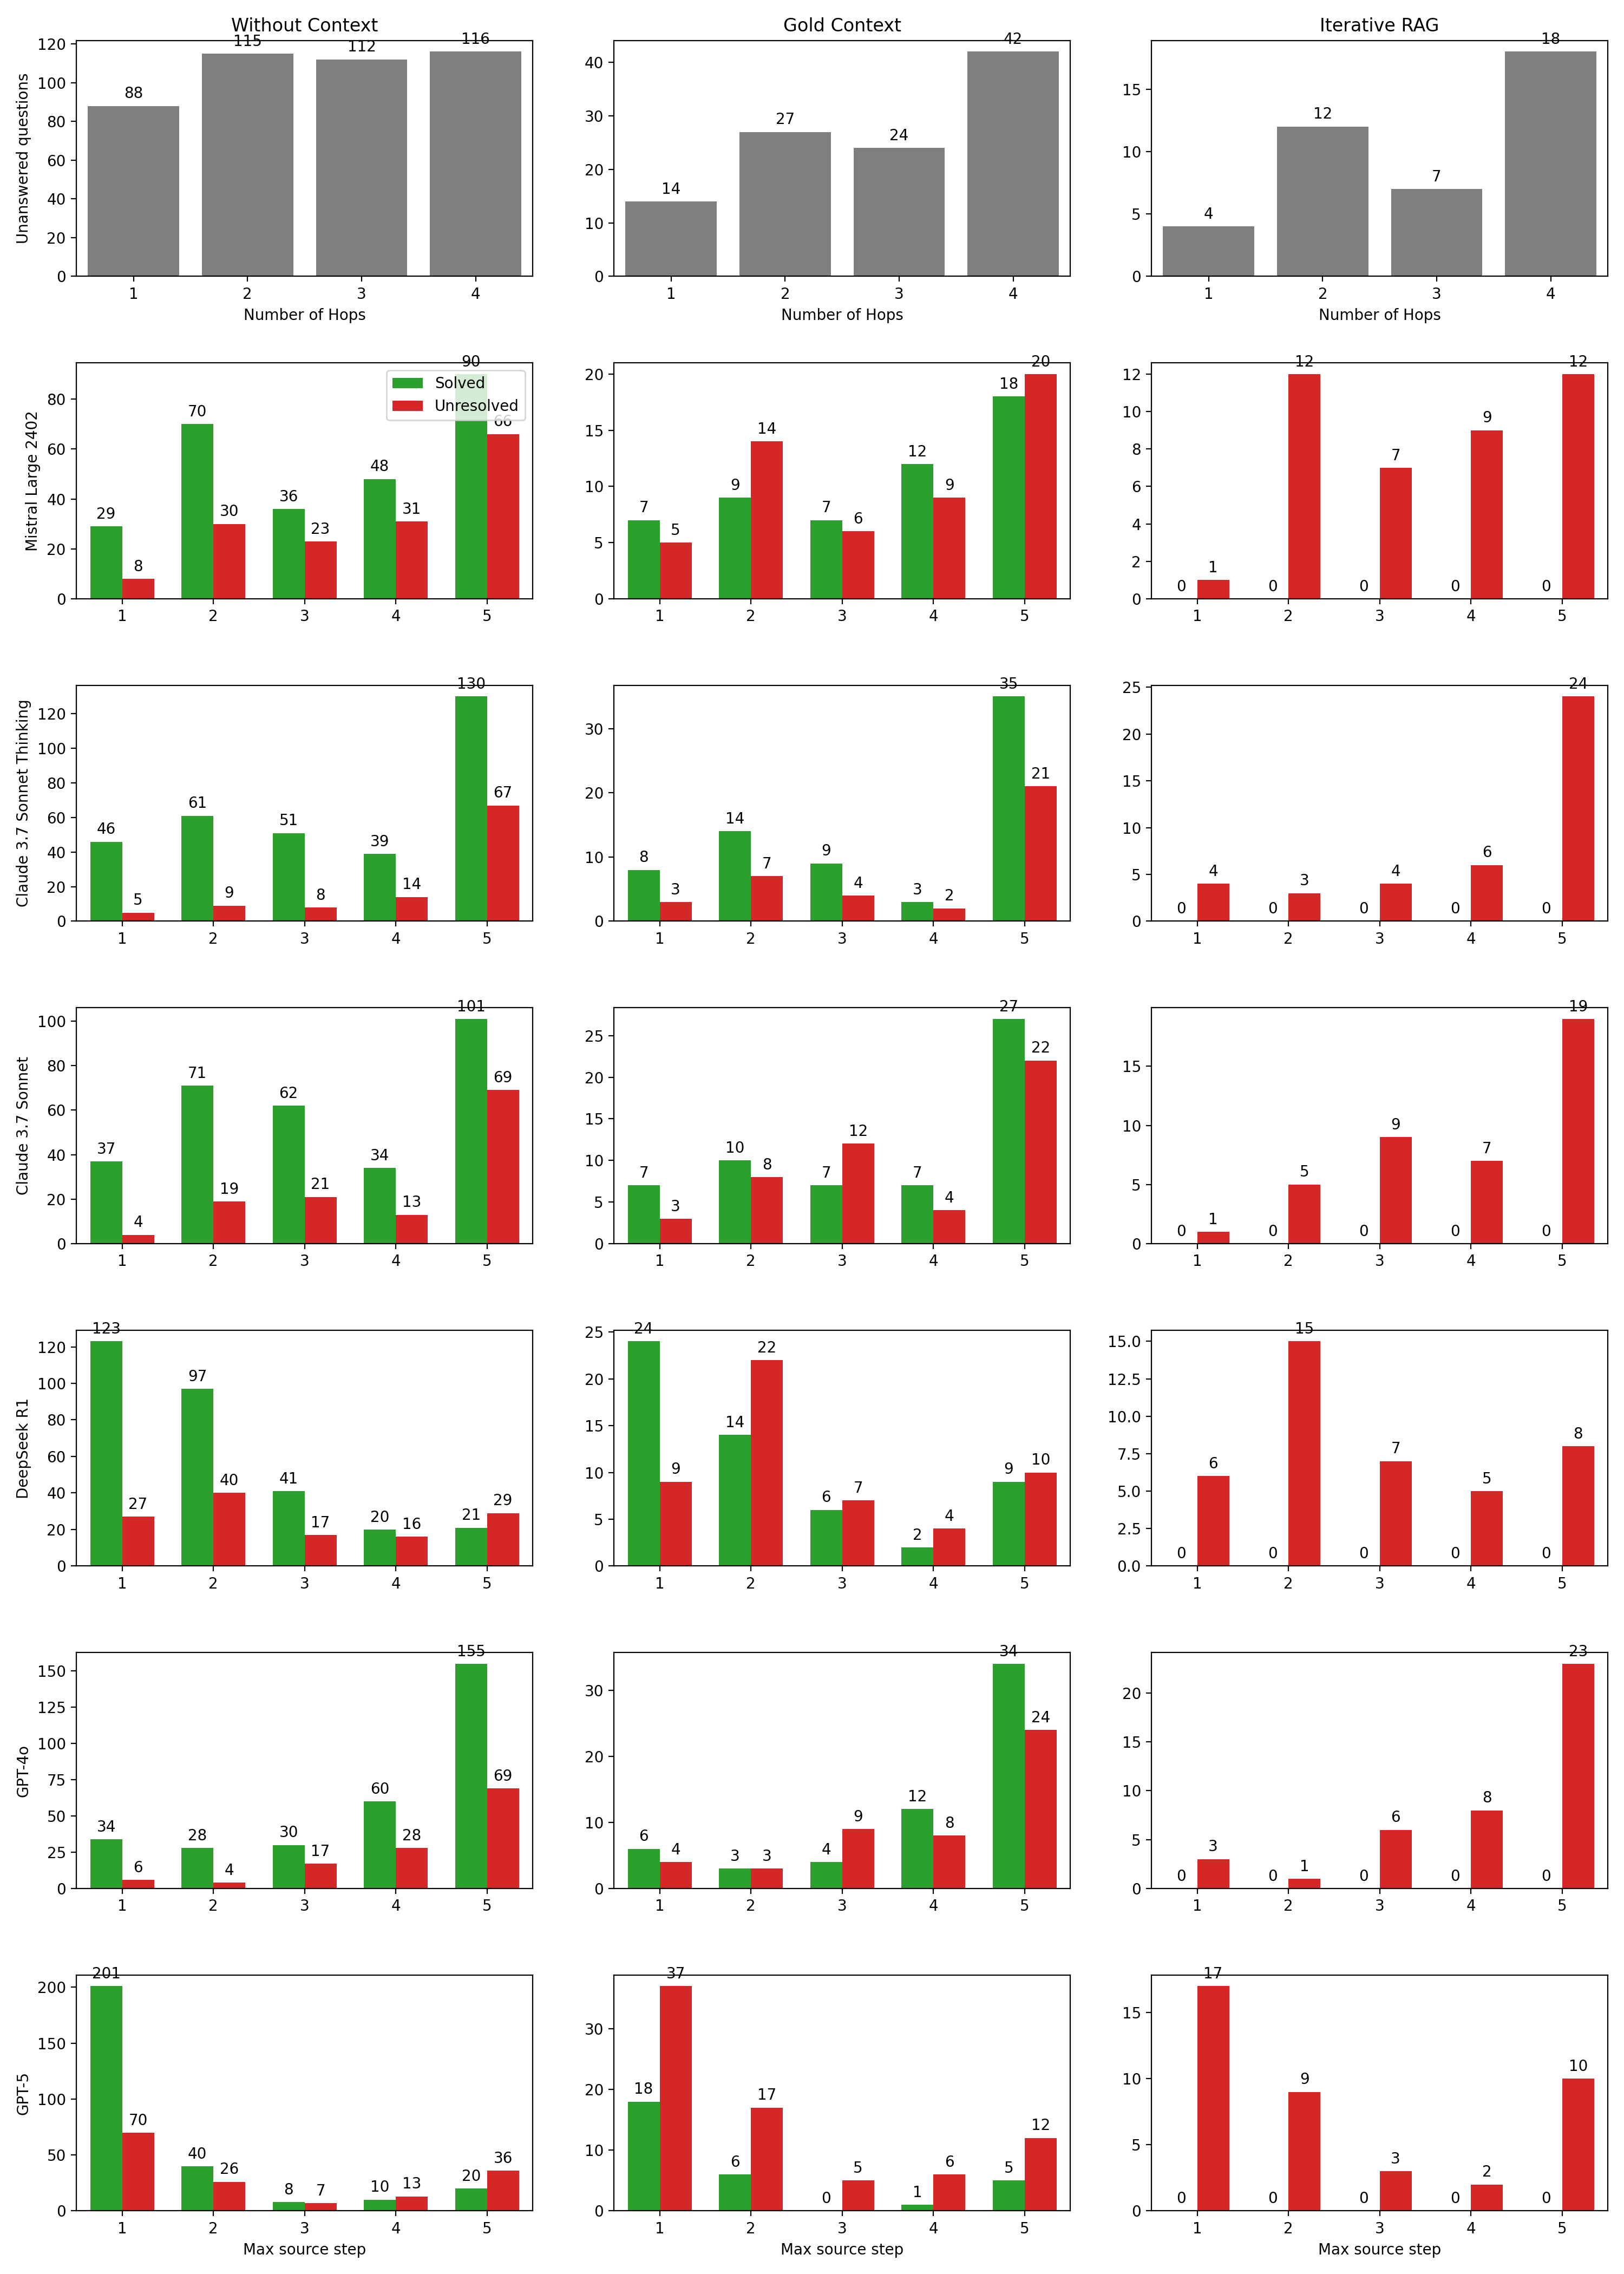
\includegraphics[width=0.85\linewidth]{src/chosen_plots/hop_distributions_all_models.png}
    \caption{Question complexity distribution by number of reasoning hops, with similar degradation trends across models as hop count increases.}
    \label{fig:hop_distributions}
\end{figure}

\subsubsection{Calibration and Confidence Patterns}

Model calibration varies substantially (Figure~\ref{fig:calibration}). We observe that models with higher well‑calibrated ("OK") shares generally realize larger iterative gains (Figure~\ref{fig:calibration_improvement}), while higher overconfidence correlates with smaller gains and more unsupported finalize decisions. The miscalibration‑by‑hop analysis (Figure~\ref{fig:miscalibration_by_hop}) shows underconfidence rising with hop complexity and overconfidence clustering where sufficiency is low—both actionable signals for gating finalize decisions and triggering additional retrieval.

\begin{figure}[t]
    \centering
    \begin{subfigure}[b]{0.48\linewidth}
        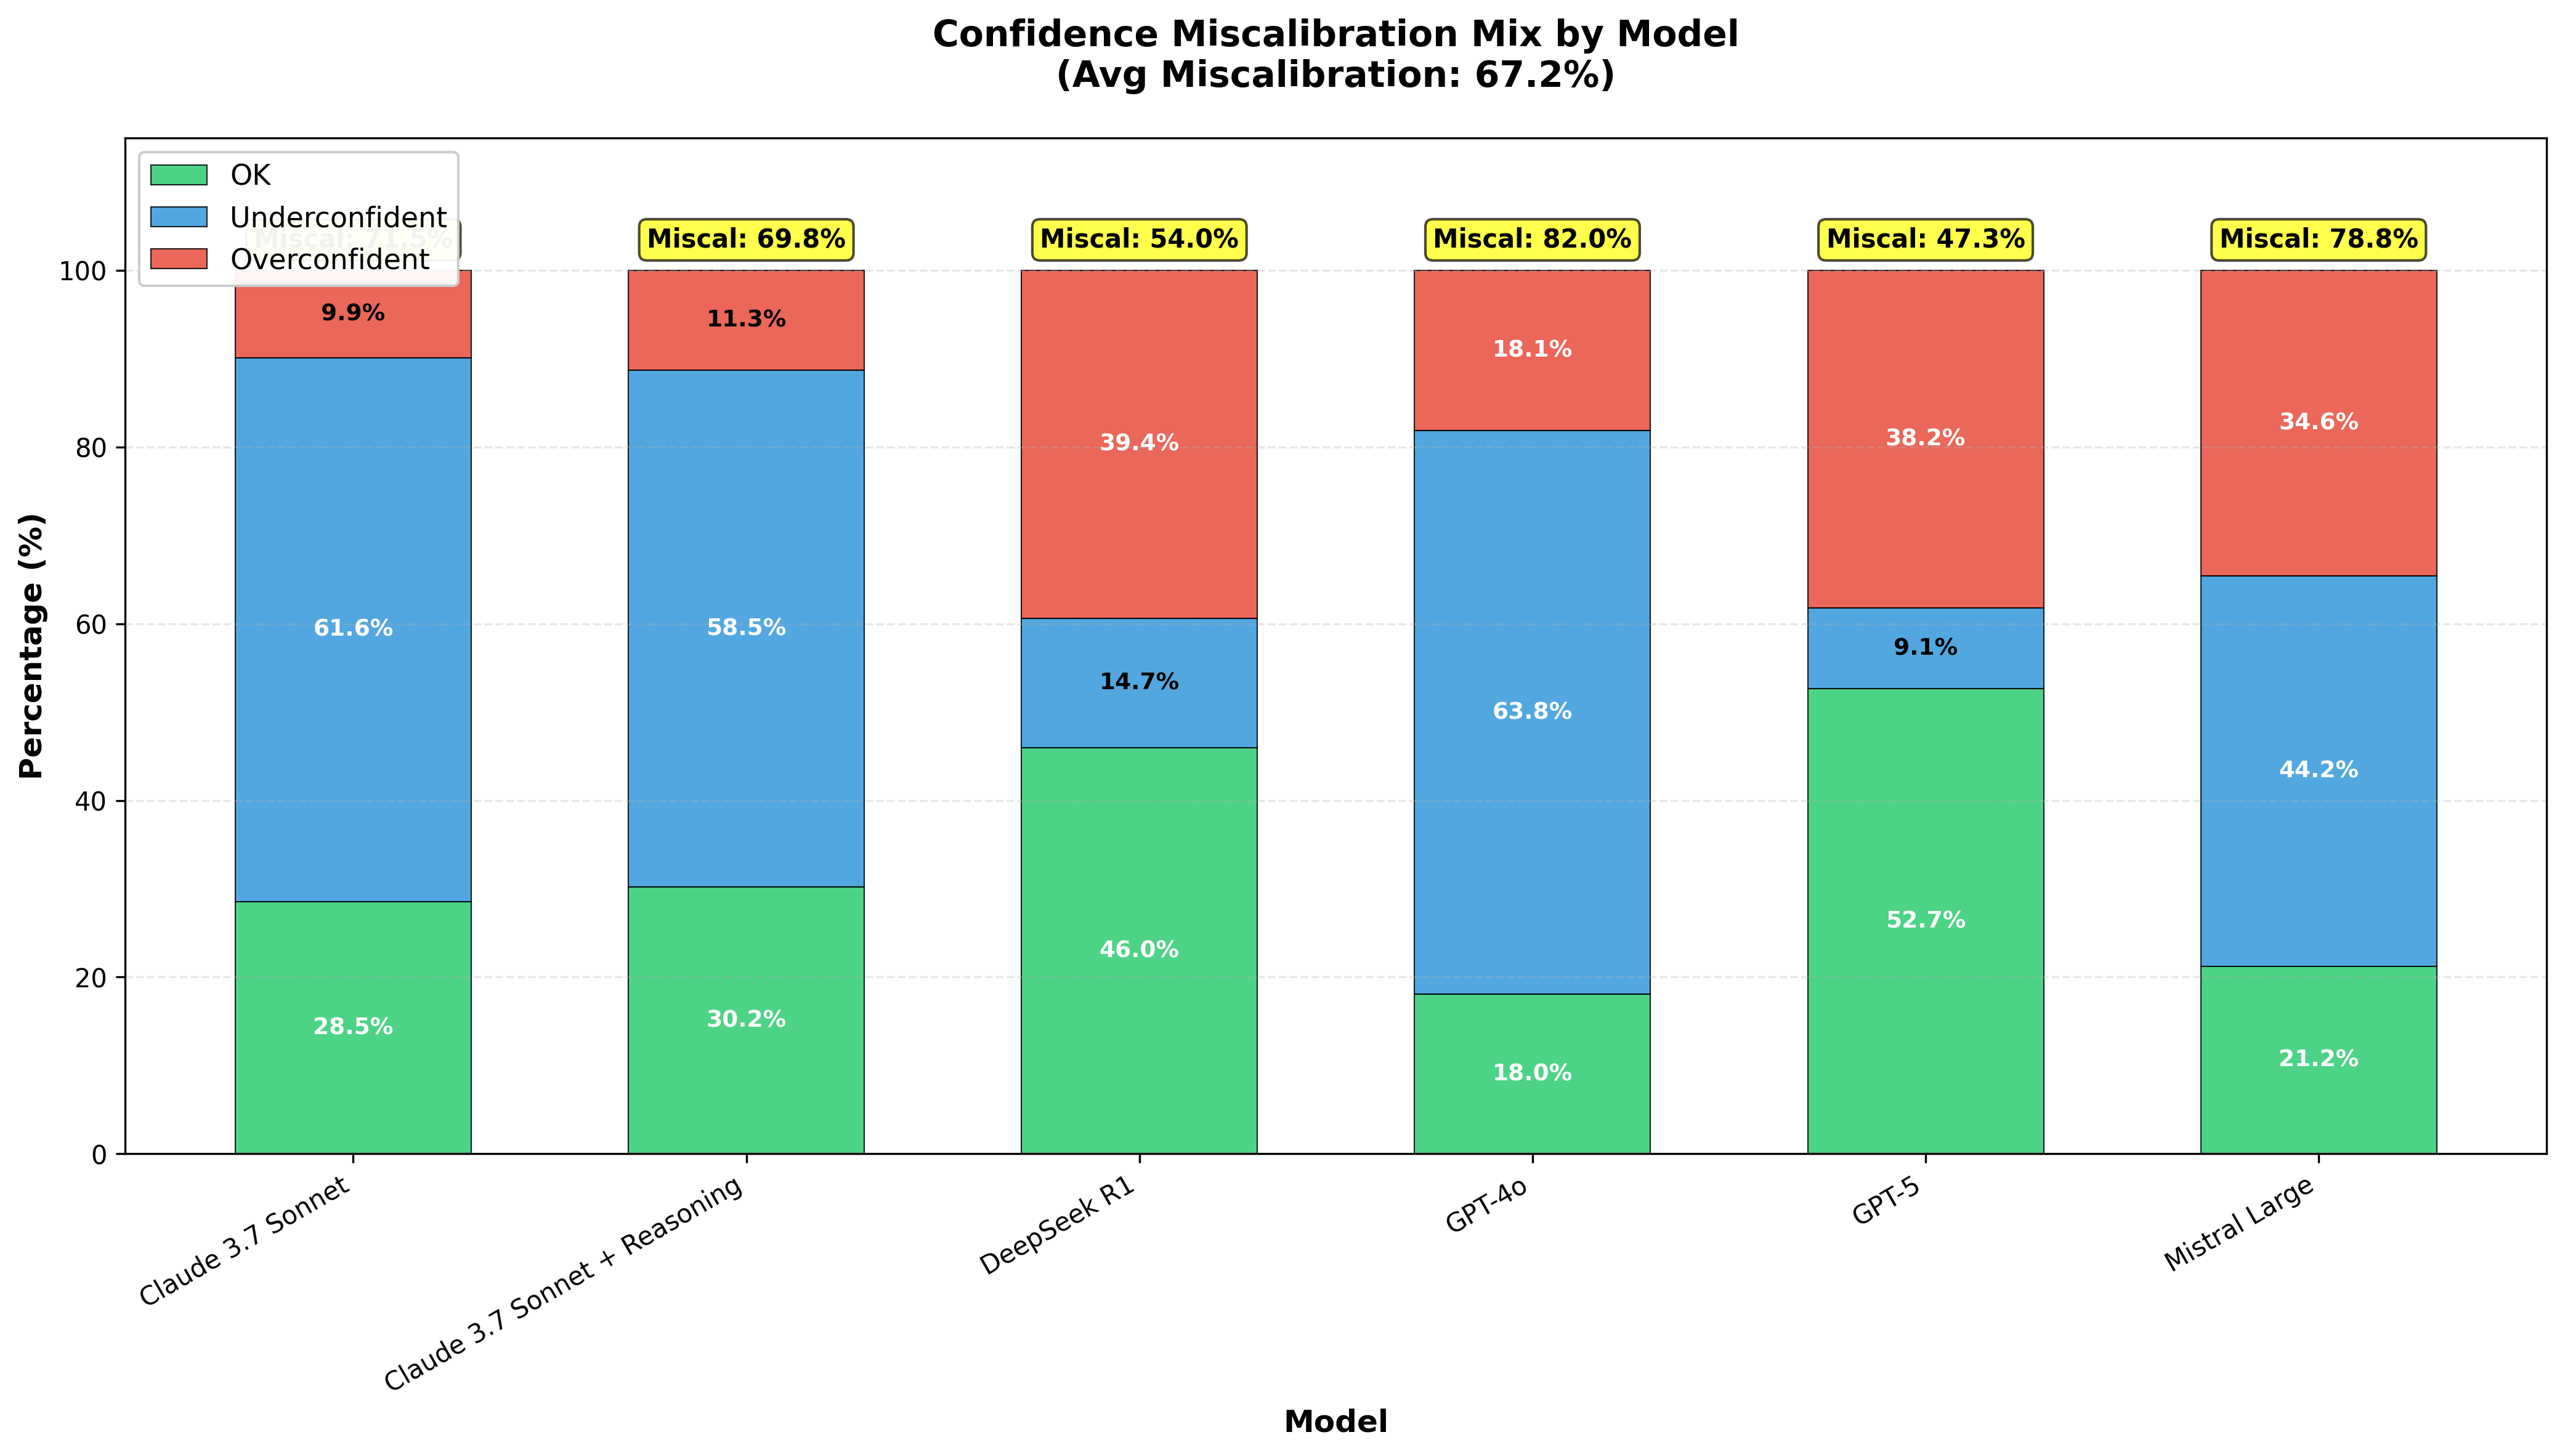
\includegraphics[width=\linewidth]{src/chosen_plots/7_miscalibration_mix.png}
        \caption{Miscalibration rates}
        \label{fig:calibration}
    \end{subfigure}
    \hfill
    \begin{subfigure}[b]{0.48\linewidth}
        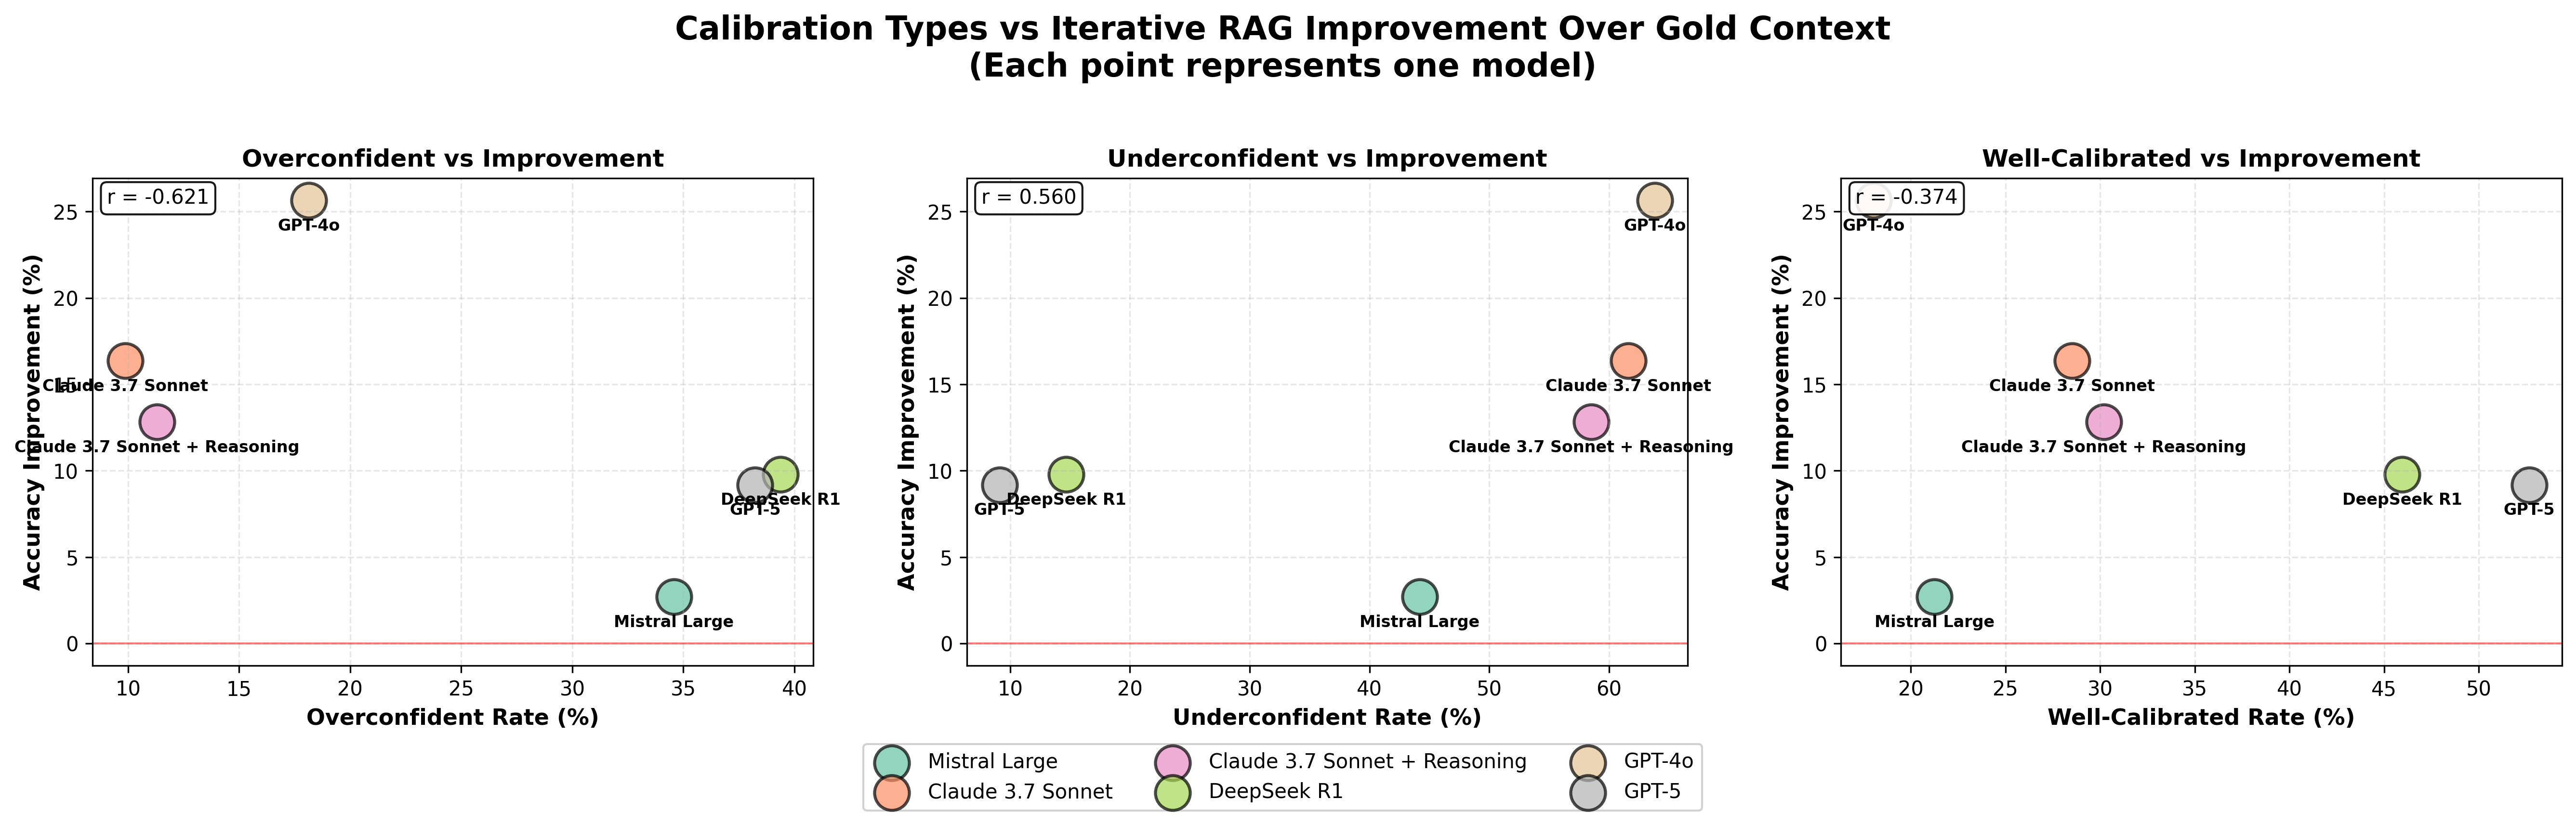
\includegraphics[width=\linewidth]{src/chosen_plots/13_calibration_combined_vs_improvement.png}
        \caption{Calibration vs. improvement}
        \label{fig:calibration_improvement}
    \end{subfigure}
    \caption{Model calibration patterns and the relationship between calibration behavior and iterative RAG improvement.}
\end{figure}

\begin{figure}[t]
    \centering
    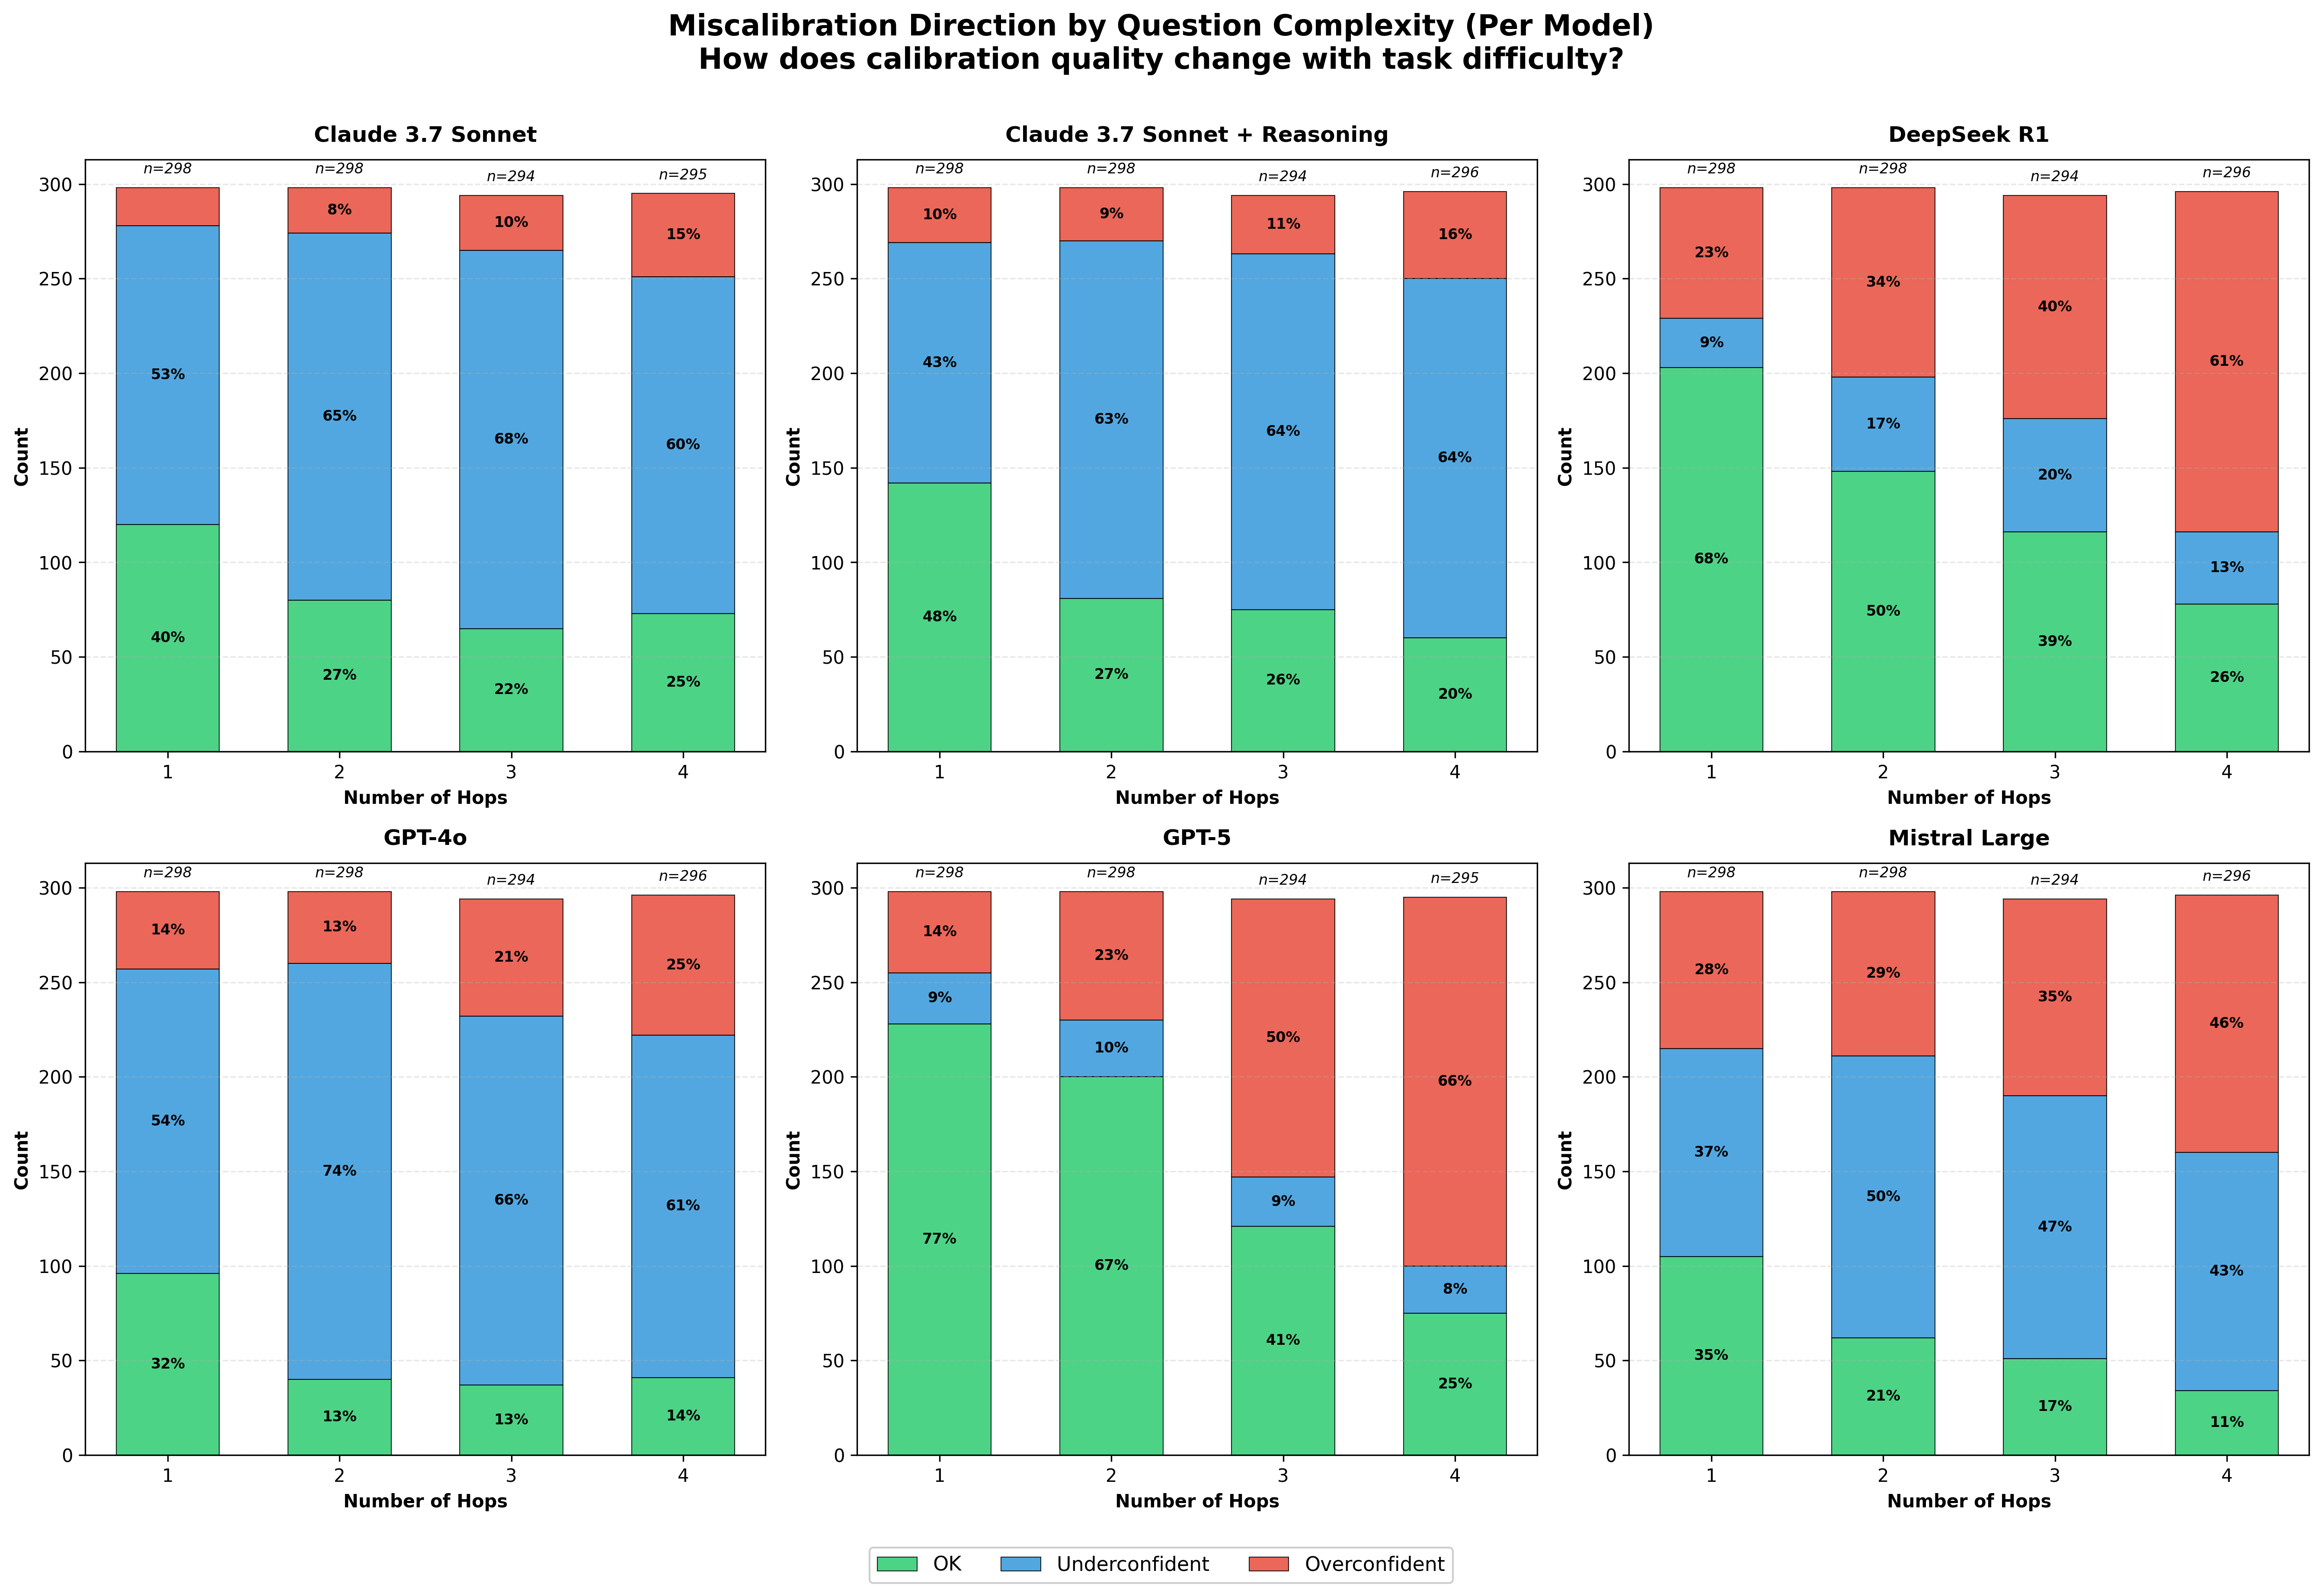
\includegraphics[width=0.8\linewidth]{src/chosen_plots/1_miscalibration_by_hop.png}
    \caption{Miscalibration by hop complexity, showing systematic overconfidence on complex questions (4+ hops) despite decreasing accuracy.}
    \label{fig:miscalibration_by_hop}
\end{figure}

\subsection{Failure Mode Analysis}

\subsubsection{Coverage Gaps as Primary Failure Mode}

Through systematic analysis of retrieval quality, we identify \textbf{coverage gaps}---situations where the system never retrieves documents needed for specific reasoning hops---as a dominant failure mode (Figure~\ref{fig:coverage_gaps}).

\paragraph{Impact Magnitude:} When coverage gaps occur, accuracy drops by large margins across models (often double‑digit percentage points). GPT‑5 is comparatively more resilient, but all systems suffer when a hop is never retrieved.

\paragraph{Prevalence:} Coverage gaps are less frequent than other issues but disproportionately affect the hardest questions, indicating retrieval difficulty scales with problem complexity.

\begin{figure}[t]
    \centering
    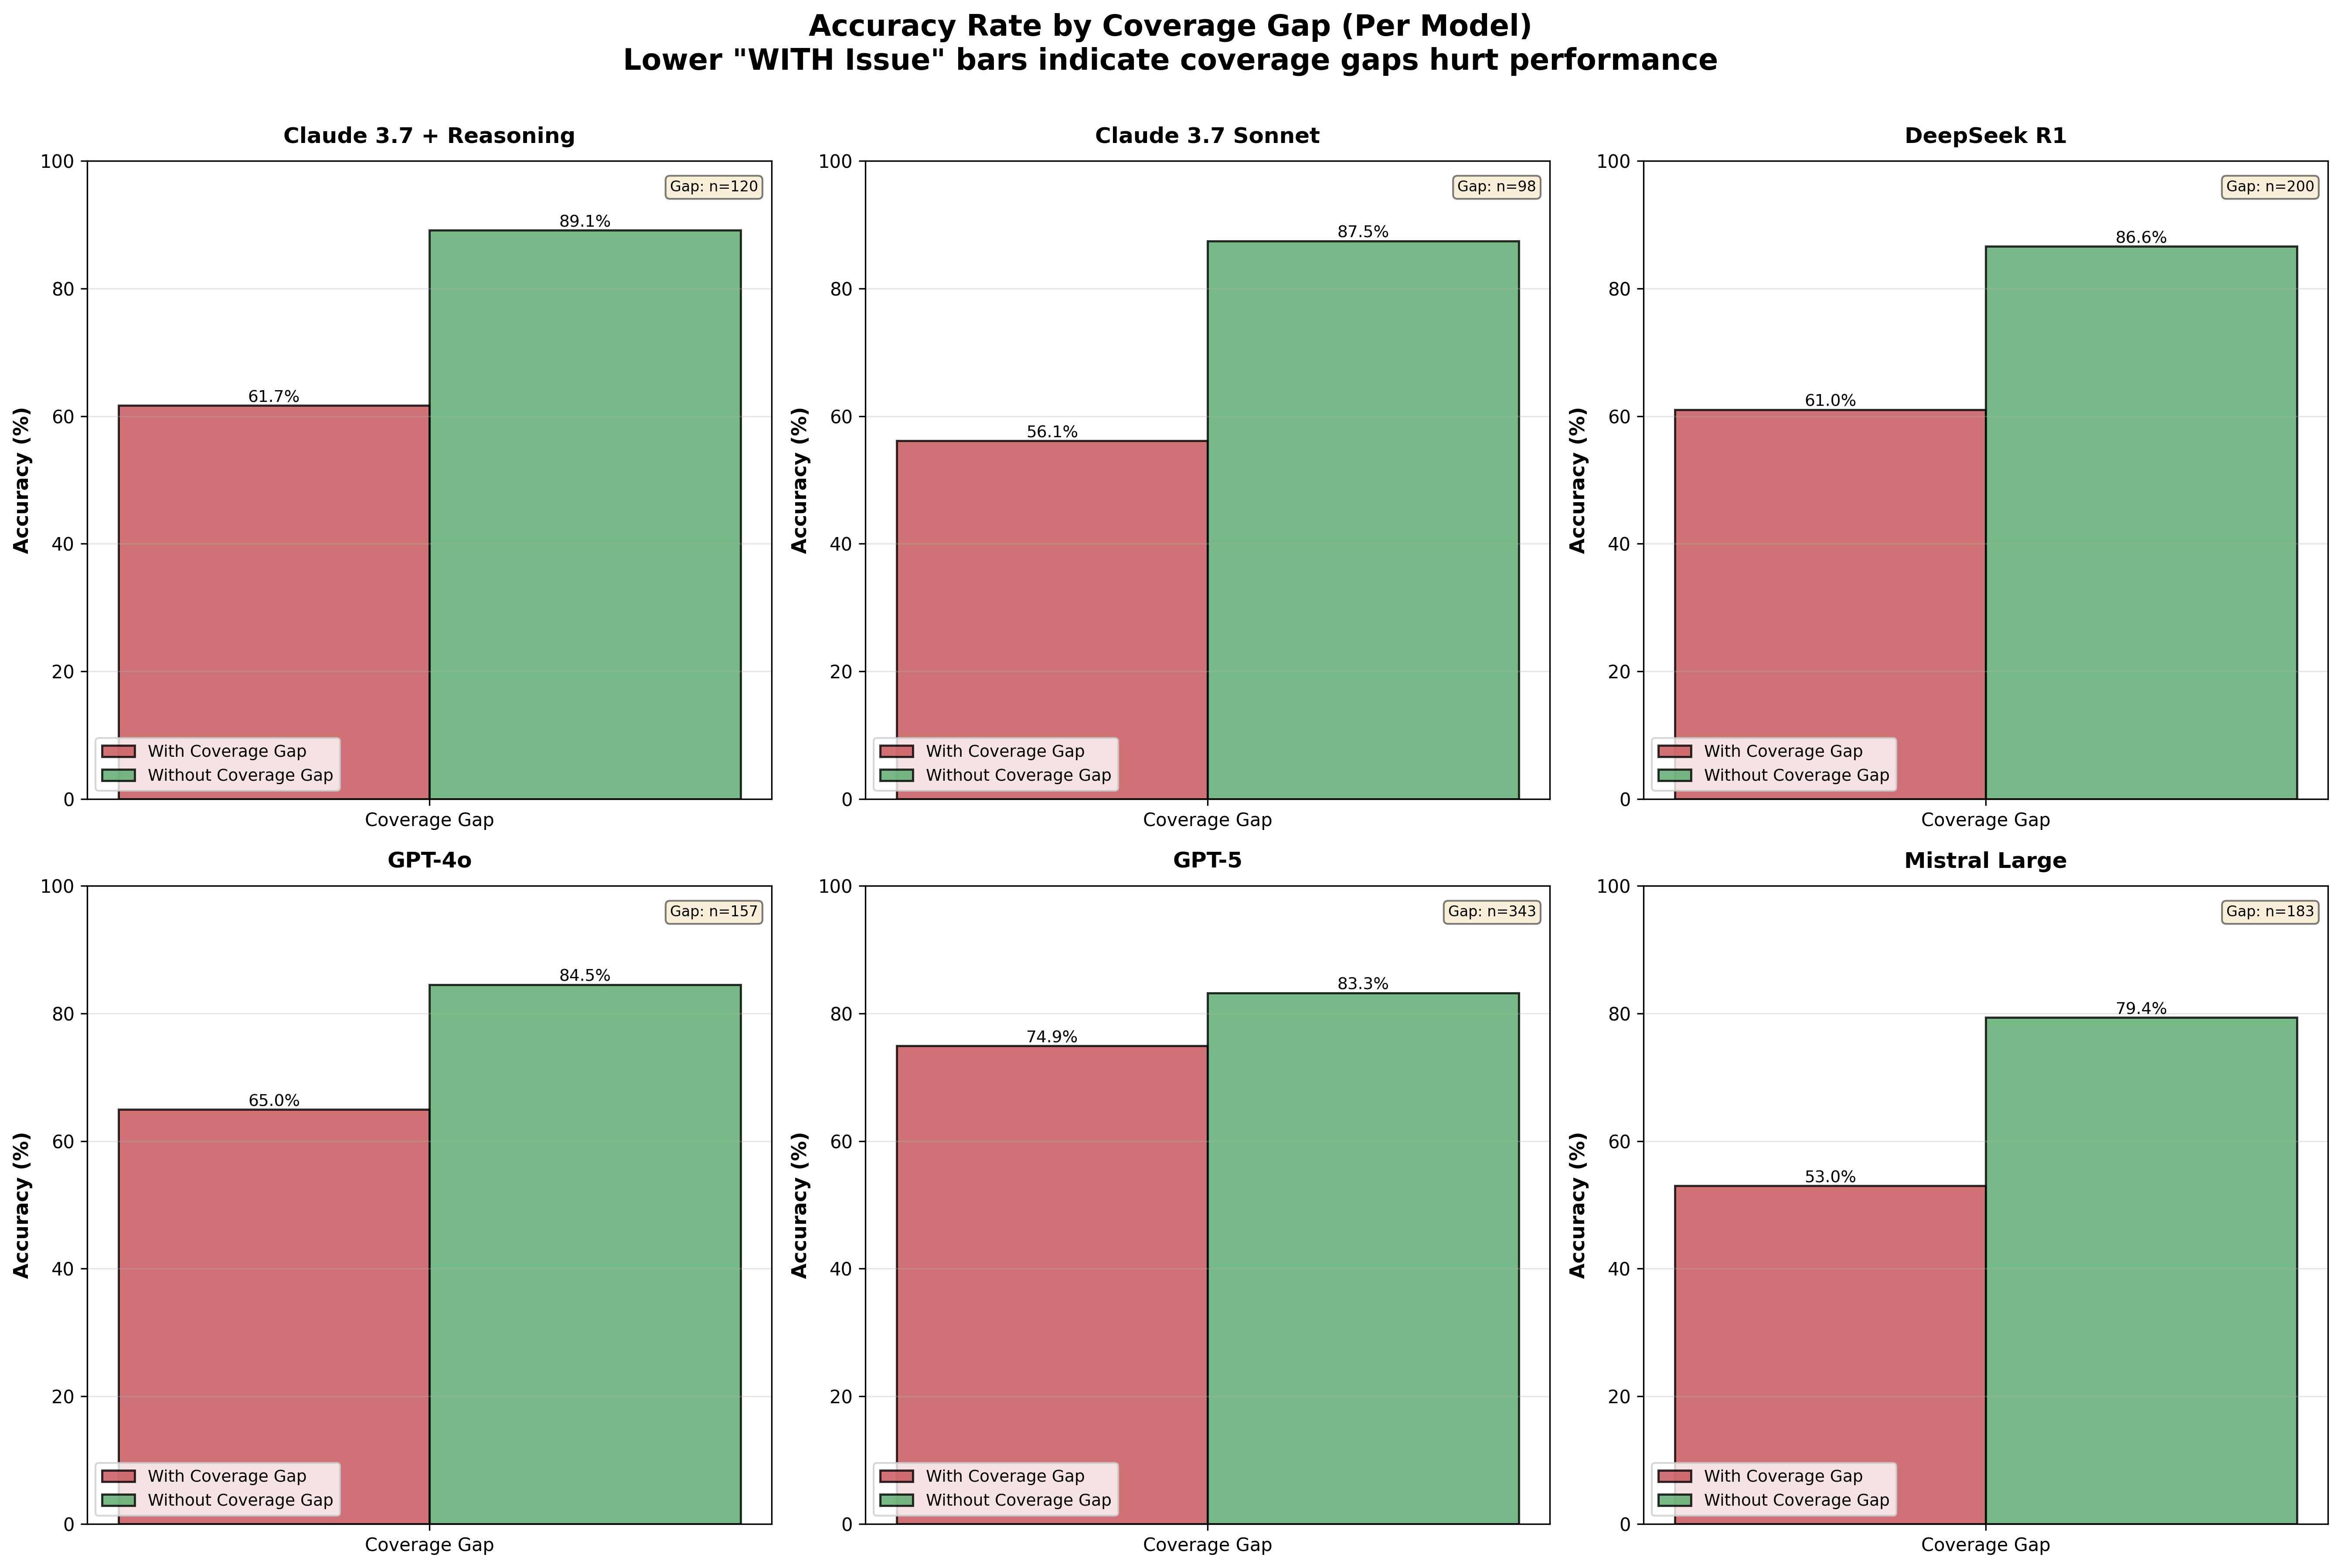
\includegraphics[width=0.95\linewidth]{src/chosen_plots/4a_accuracy_by_issue_per_model_coverage_only.png}
    \caption{Accuracy with vs. without coverage gaps across models. Coverage gaps substantially reduce accuracy; GPT‑5 shows comparatively higher resilience.}
    \label{fig:coverage_gaps}
\end{figure}

\subsubsection{Missed Hop Patterns}

Detailed analysis of which hops are missed reveals systematic patterns (Figure~\ref{fig:missed_hops}):

\paragraph{Hop 1 (Foundation Hop):} Most consequential when missed
\begin{itemize}
    \item Failure here often leads to a cascade (later hops are more likely to be missed)
    \item Often tied to ambiguous entity references or specialized terminology
\end{itemize}

\paragraph{Hop 2 (Bridging Hop):}
\begin{itemize}
    \item Often requires integration of Hop 1 information to formulate the correct query
    \item Models can struggle with query reformulation based on partial information
\end{itemize}

\paragraph{Hop 3+ (Extended Reasoning):}
\begin{itemize}
    \item Retrieval difficulty increases with hop depth; distractor latch becomes more common
\end{itemize}

\textbf{Key Insight}: The system exhibits a ``failure cascade'' pattern. When Hop 1 is missed, probability of missing subsequent hops rises sharply. This suggests that error recovery mechanisms should focus on early-stage retrieval quality.

\begin{figure}[t]
    \centering
    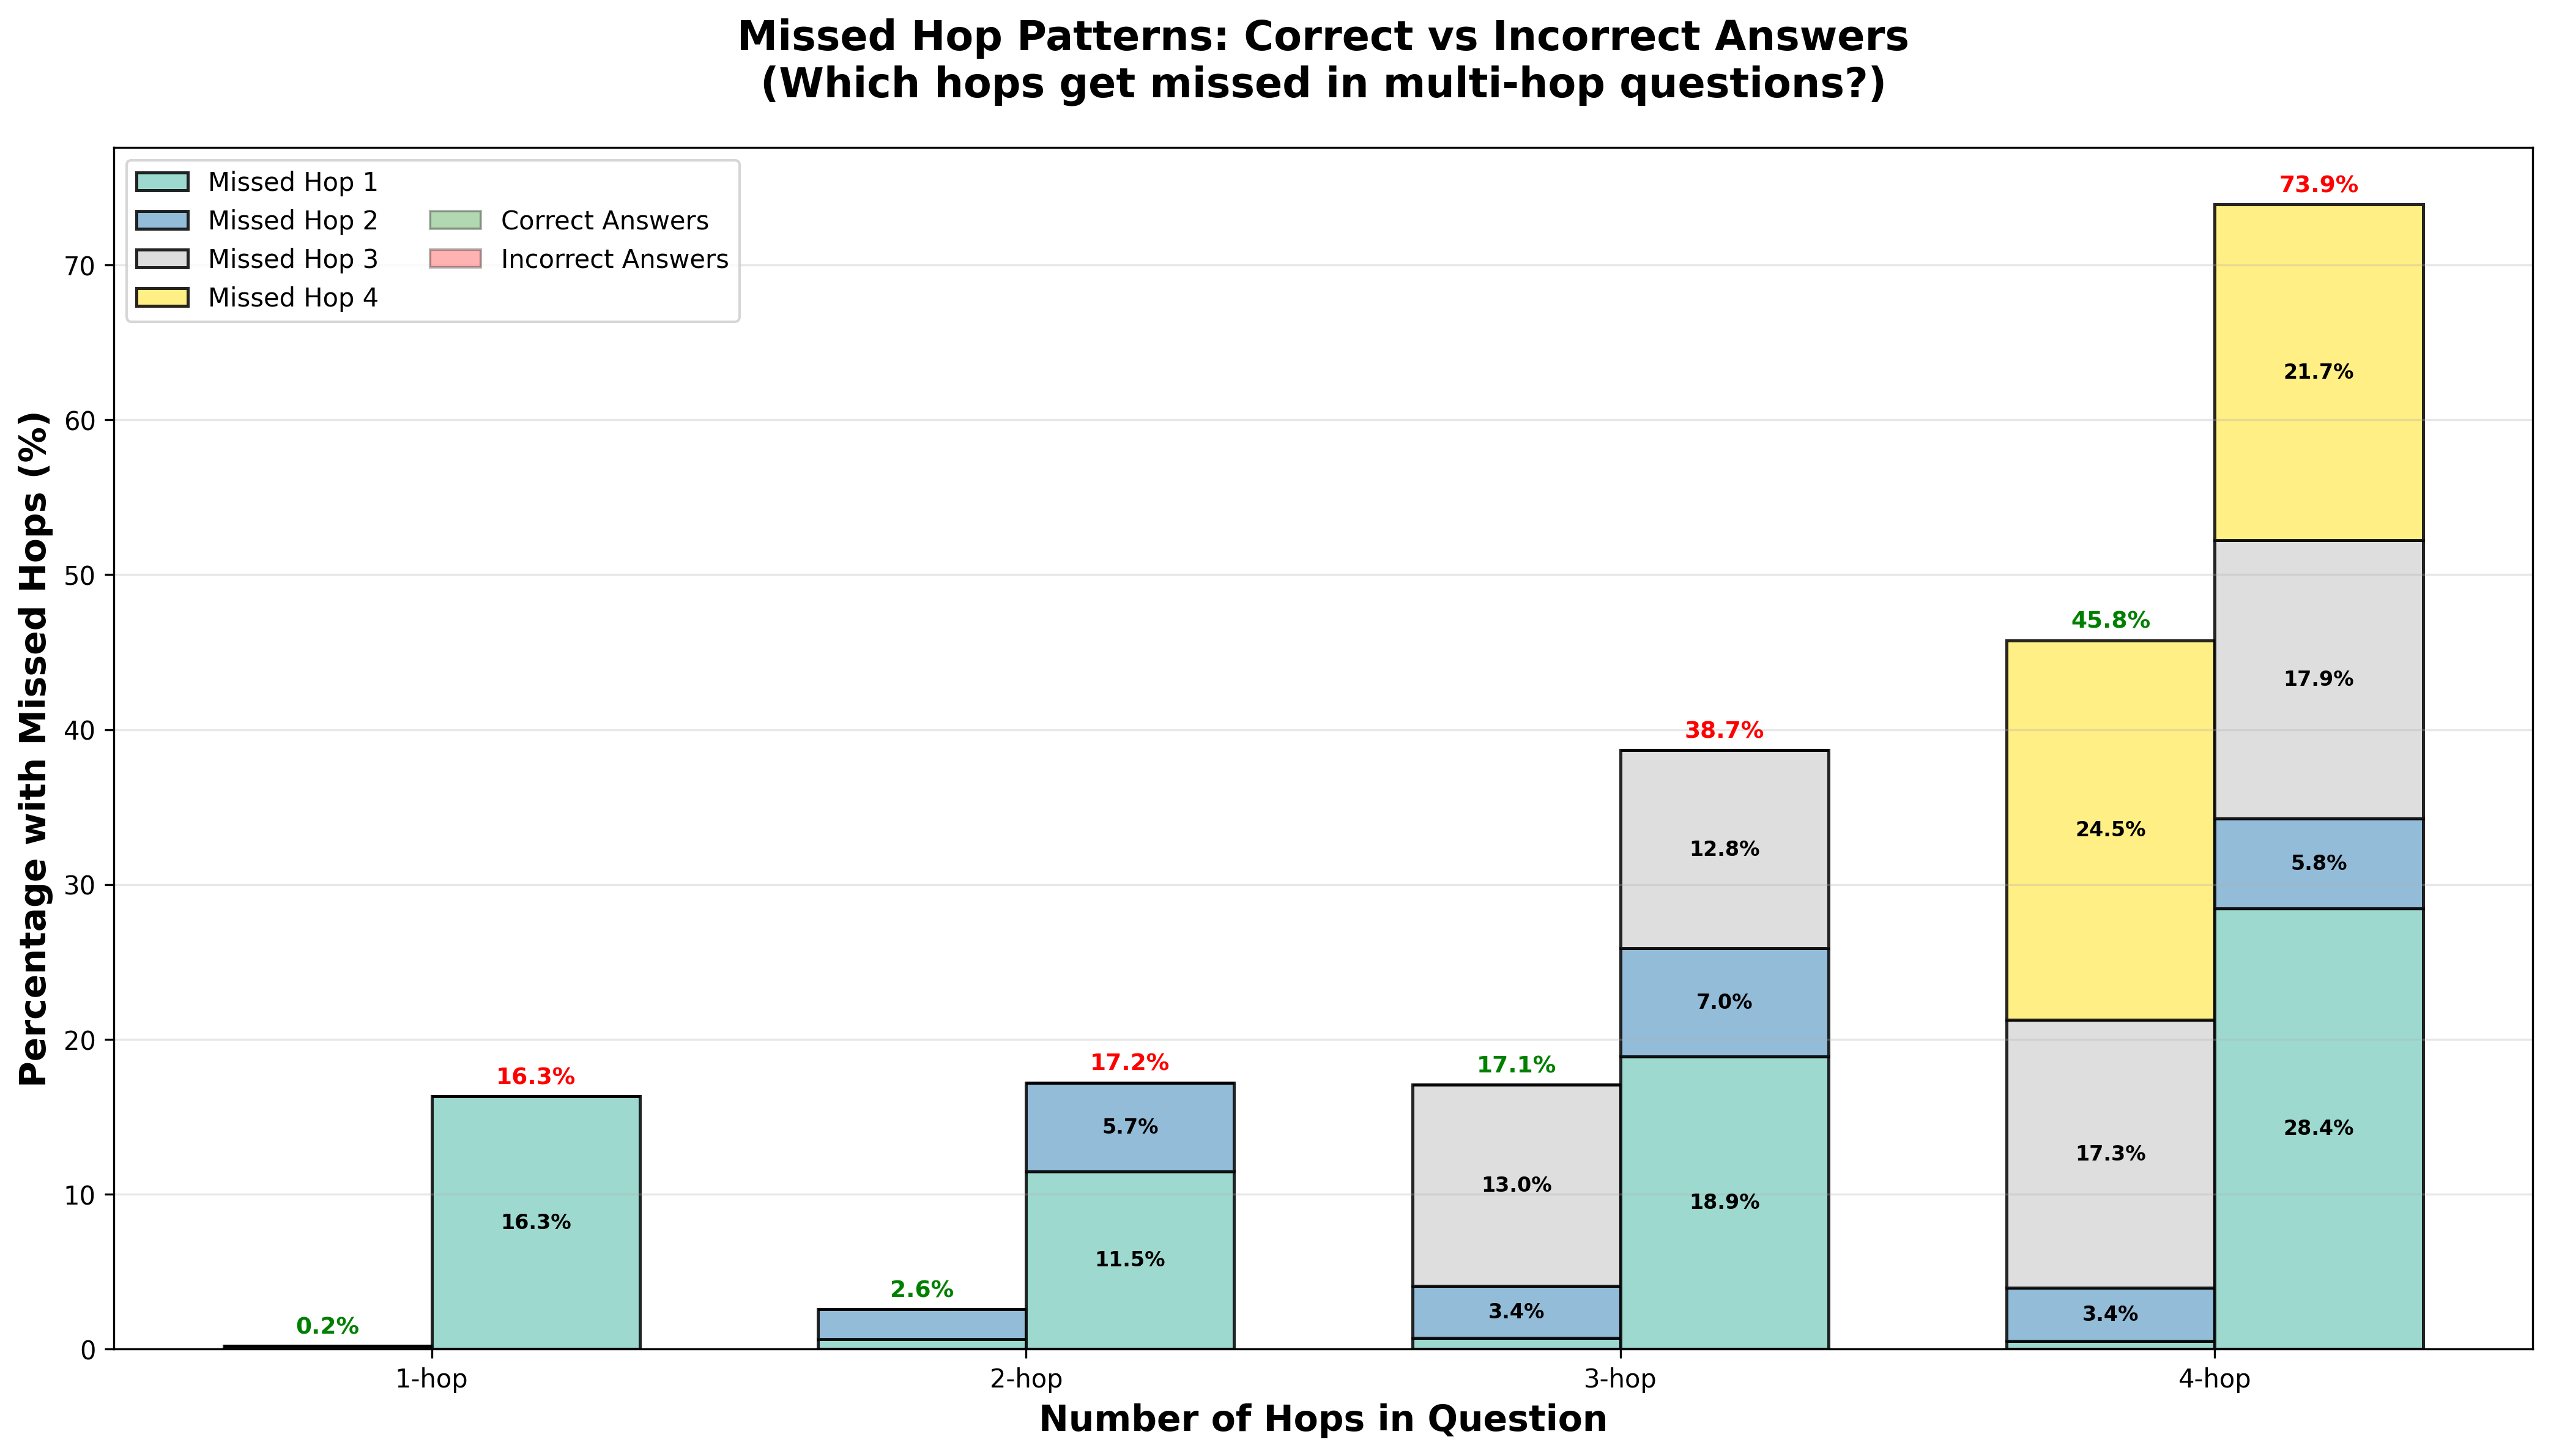
\includegraphics[width=0.8\linewidth]{src/chosen_plots/missed_hop_patterns.png}
    \caption{Missed hop patterns showing systematic failure cascade where Hop 1 misses increase probability of subsequent hop failures by 3--5$\times$.}
    \label{fig:missed_hops}
\end{figure}

\subsubsection{Composition Failures}

Composition failures---where the model fails to correctly integrate information across retrieved documents---are observed across models (Figure~\ref{fig:composition_failures}).

\paragraph{Variation by Model:} Some models are more prone to composition failures than others; the distribution aligns with calibration profiles and evidence sufficiency trends.

\paragraph{Root Cause Analysis:} Composition failures co-occur with retrieval issues (coverage gaps or late hits) and poor query quality; both reduce sufficiency and increase the odds of overconfident finalize decisions.

Notably, composition failures track closely with evidence sufficiency (Figure~\ref{fig:sufficiency}). A sufficiency threshold to gate finalize decisions (e.g., avoiding finalize when sufficiency is low) can prevent many overconfident errors and allow further retrieval/refinement.

\begin{figure}[t]
    \centering
    \begin{subfigure}[b]{0.48\linewidth}
        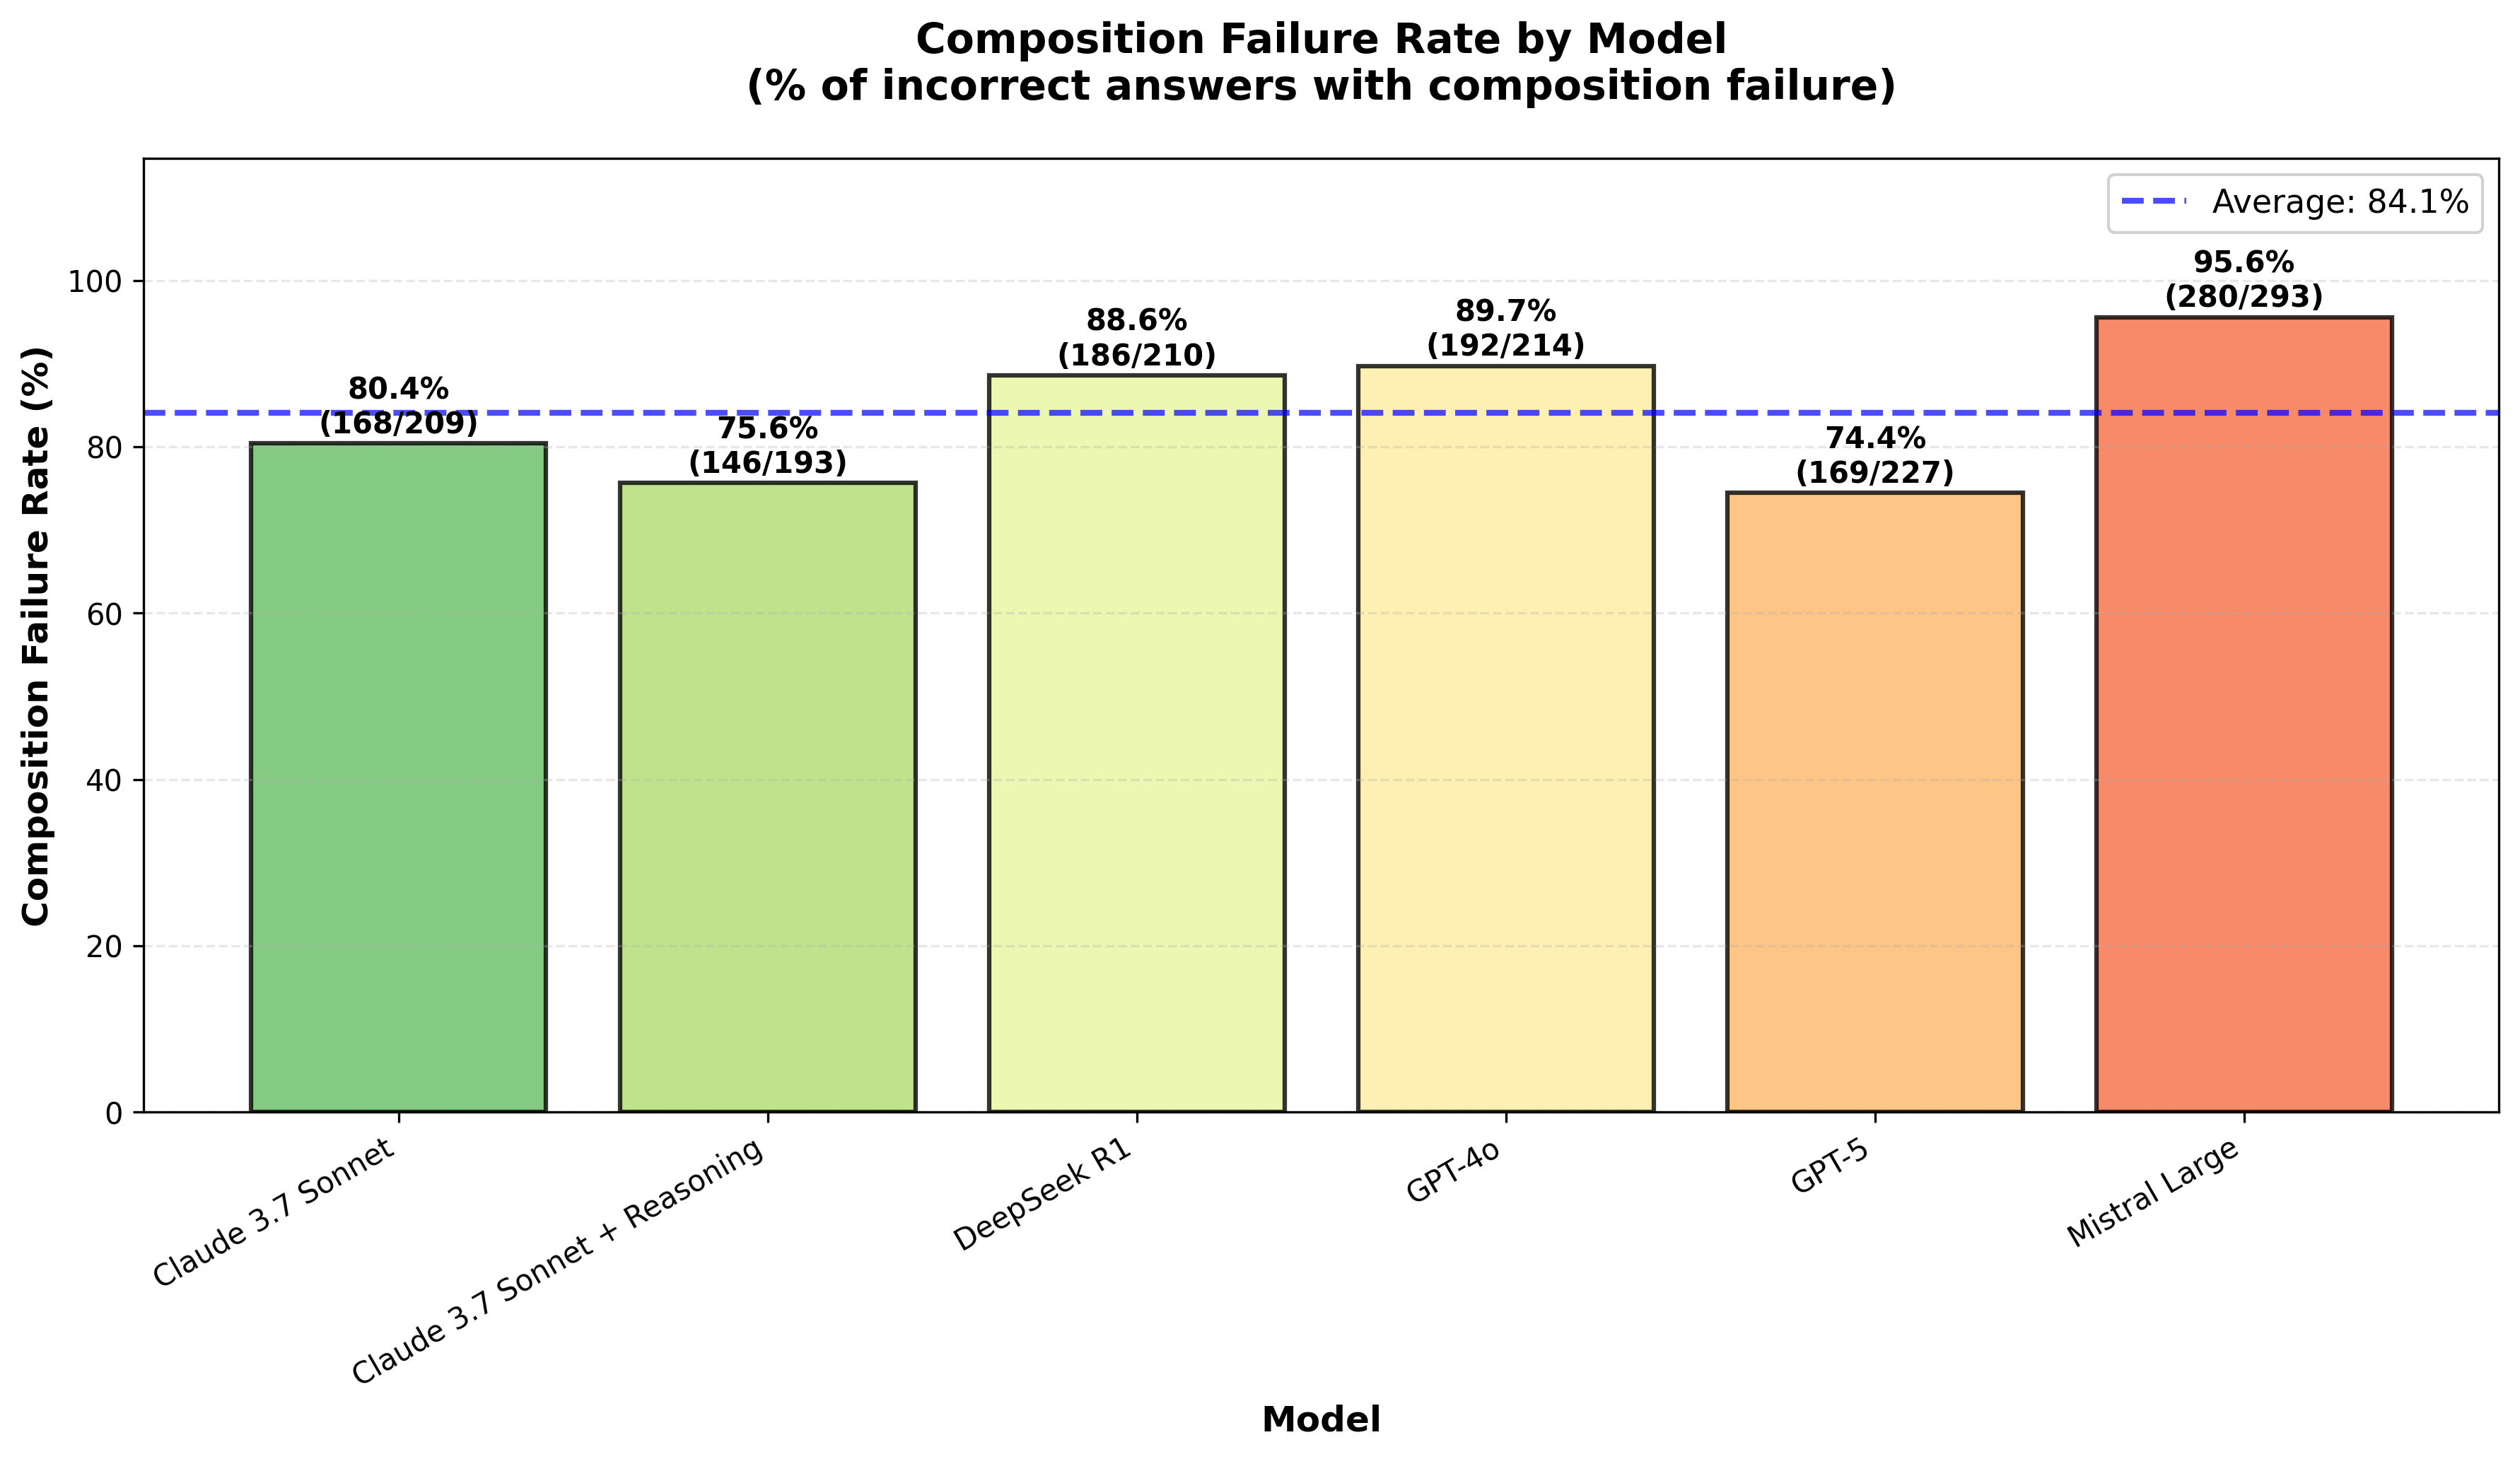
\includegraphics[width=\linewidth]{src/chosen_plots/5_composition_failure_rate.png}
        \caption{Composition failure rates}
        \label{fig:composition_failures}
    \end{subfigure}
    \hfill
    \begin{subfigure}[b]{0.48\linewidth}
        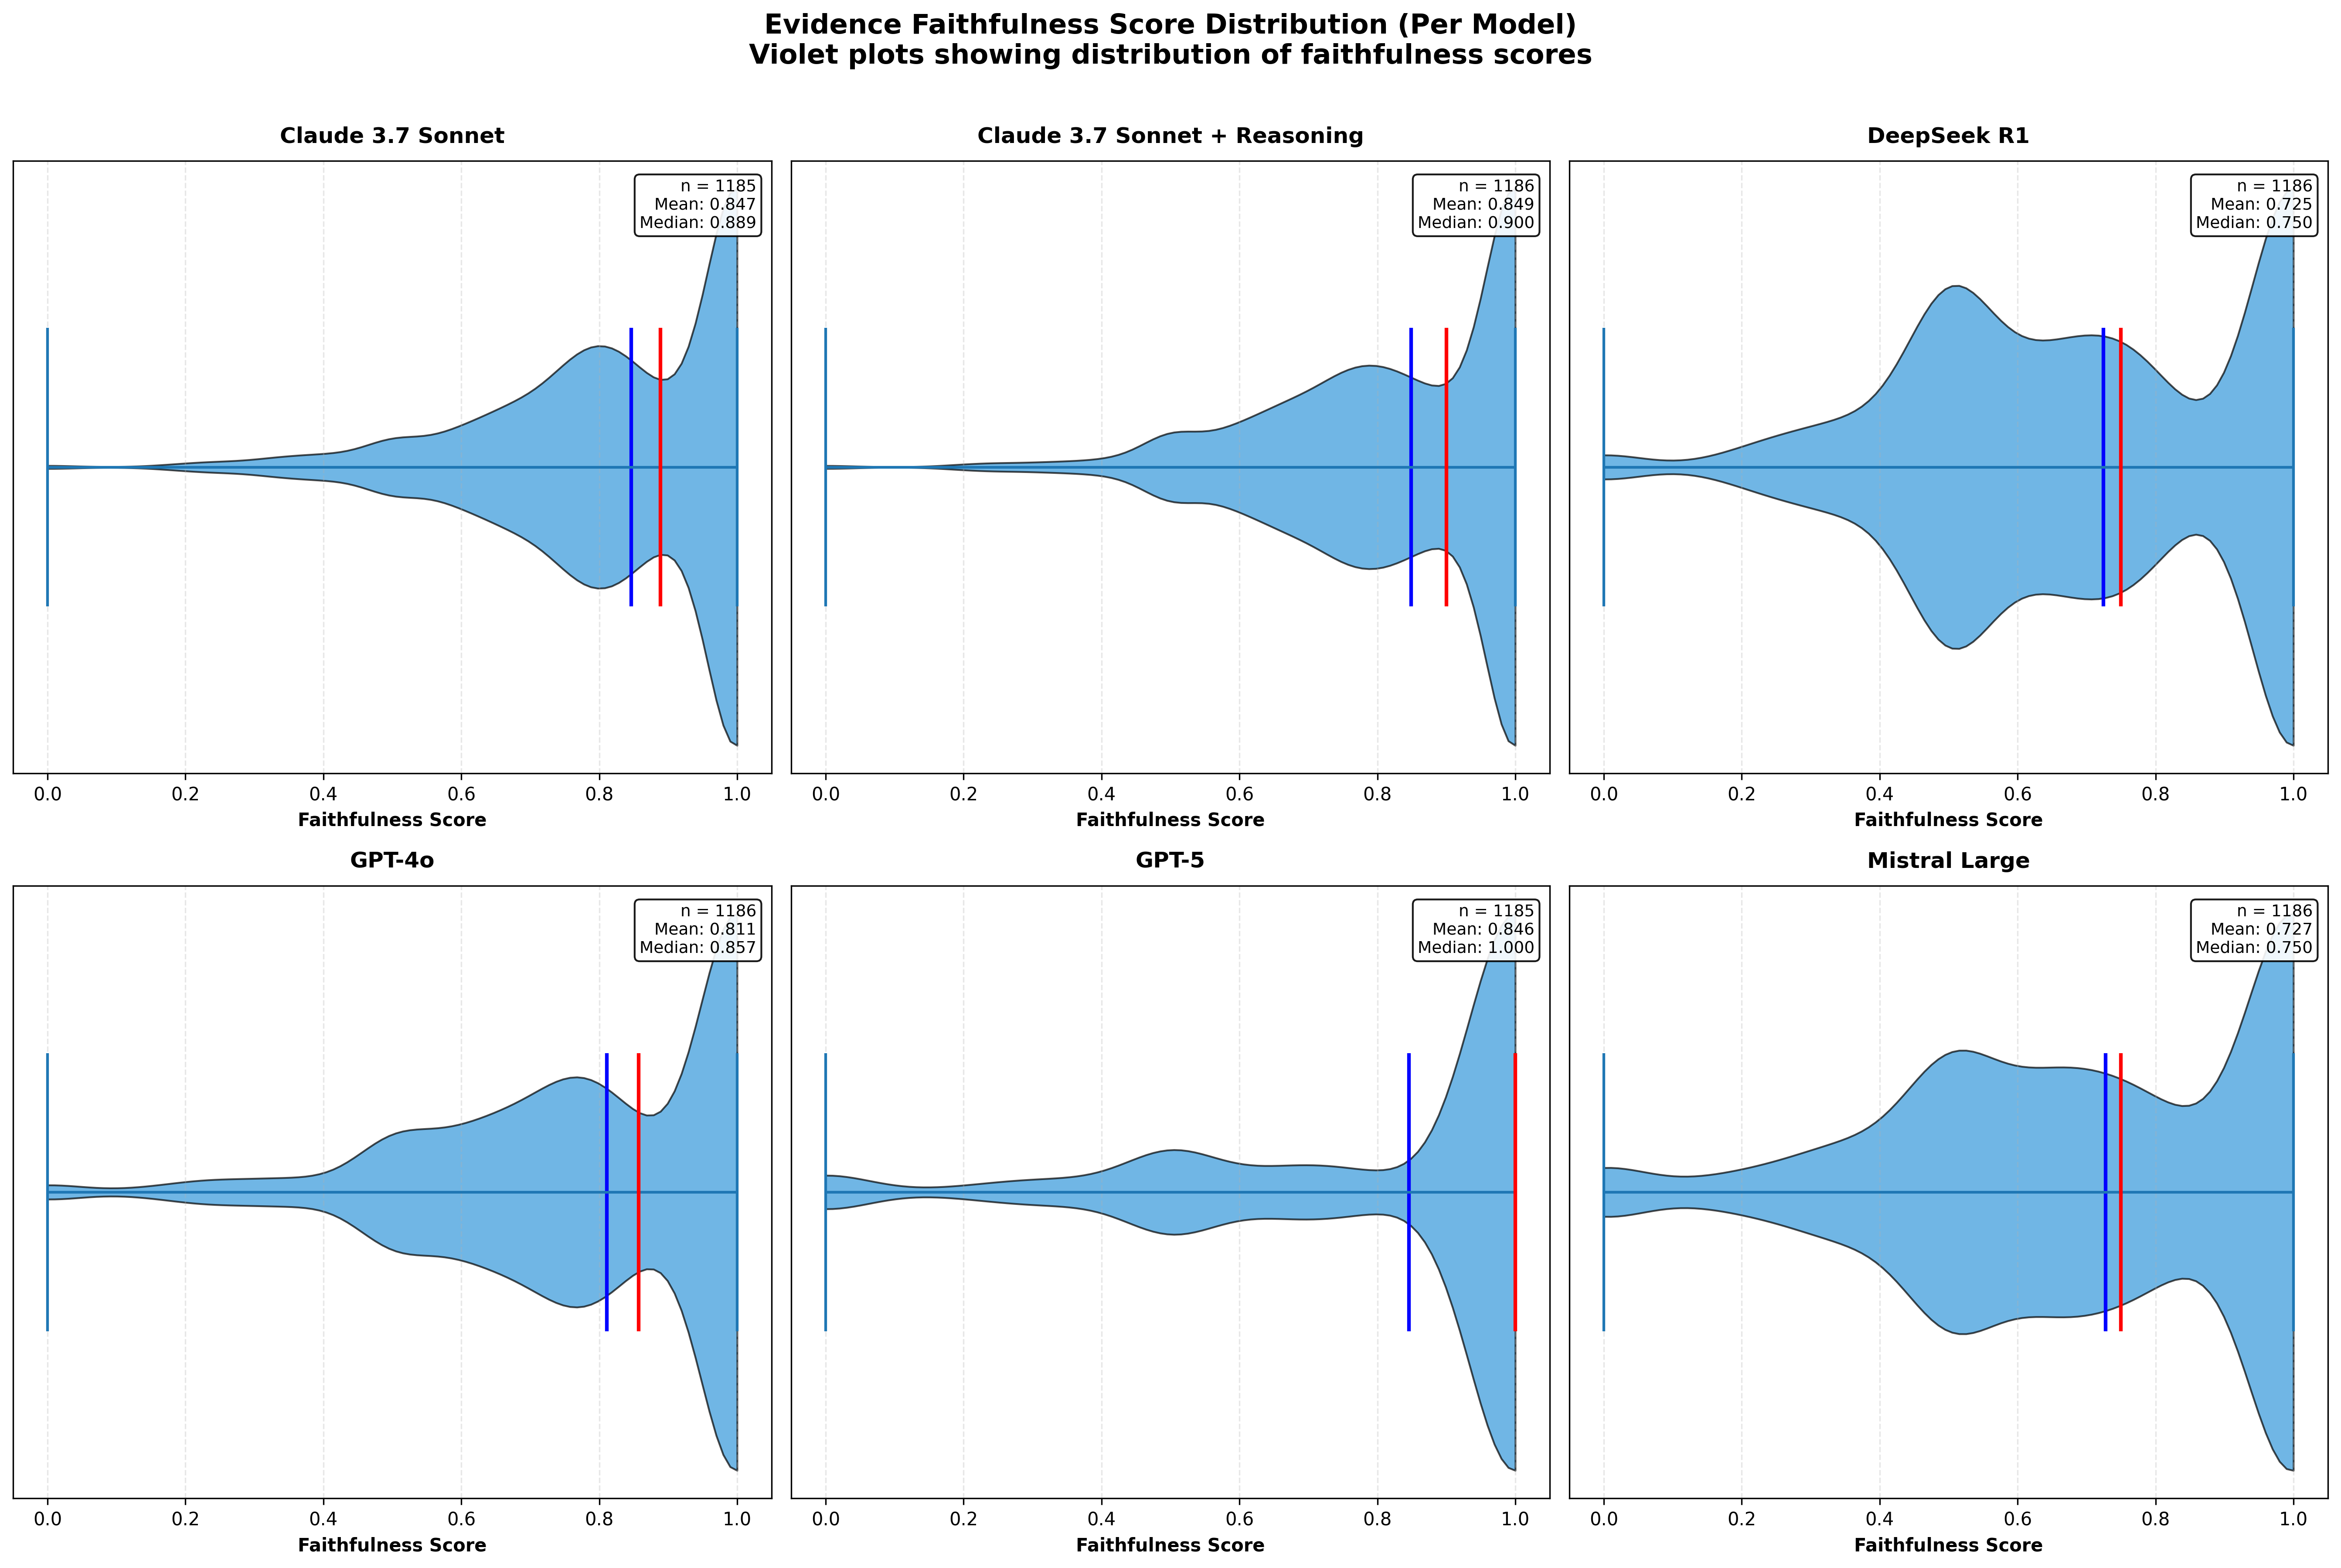
\includegraphics[width=\linewidth]{src/chosen_plots/6_sufficiency_distribution.png}
        \caption{Evidence sufficiency distribution}
        \label{fig:sufficiency}
    \end{subfigure}
    \caption{Composition failures correlate strongly with evidence sufficiency; thresholding finalize by sufficiency helps prevent overconfident errors.}
\end{figure}

\subsubsection{Faithfulness and Hallucination Patterns}

Analysis of faithfulness reveals important patterns (Figure~\ref{fig:faithfulness}). Overconfidence concentrates where coverage is high but sufficiency is low (the "danger zone"), producing unsupported claims and composition failures. Conversely, when sufficiency is high, models tend to remain calibrated and accurate even as coverage varies.

\begin{figure}[t]
    \centering
    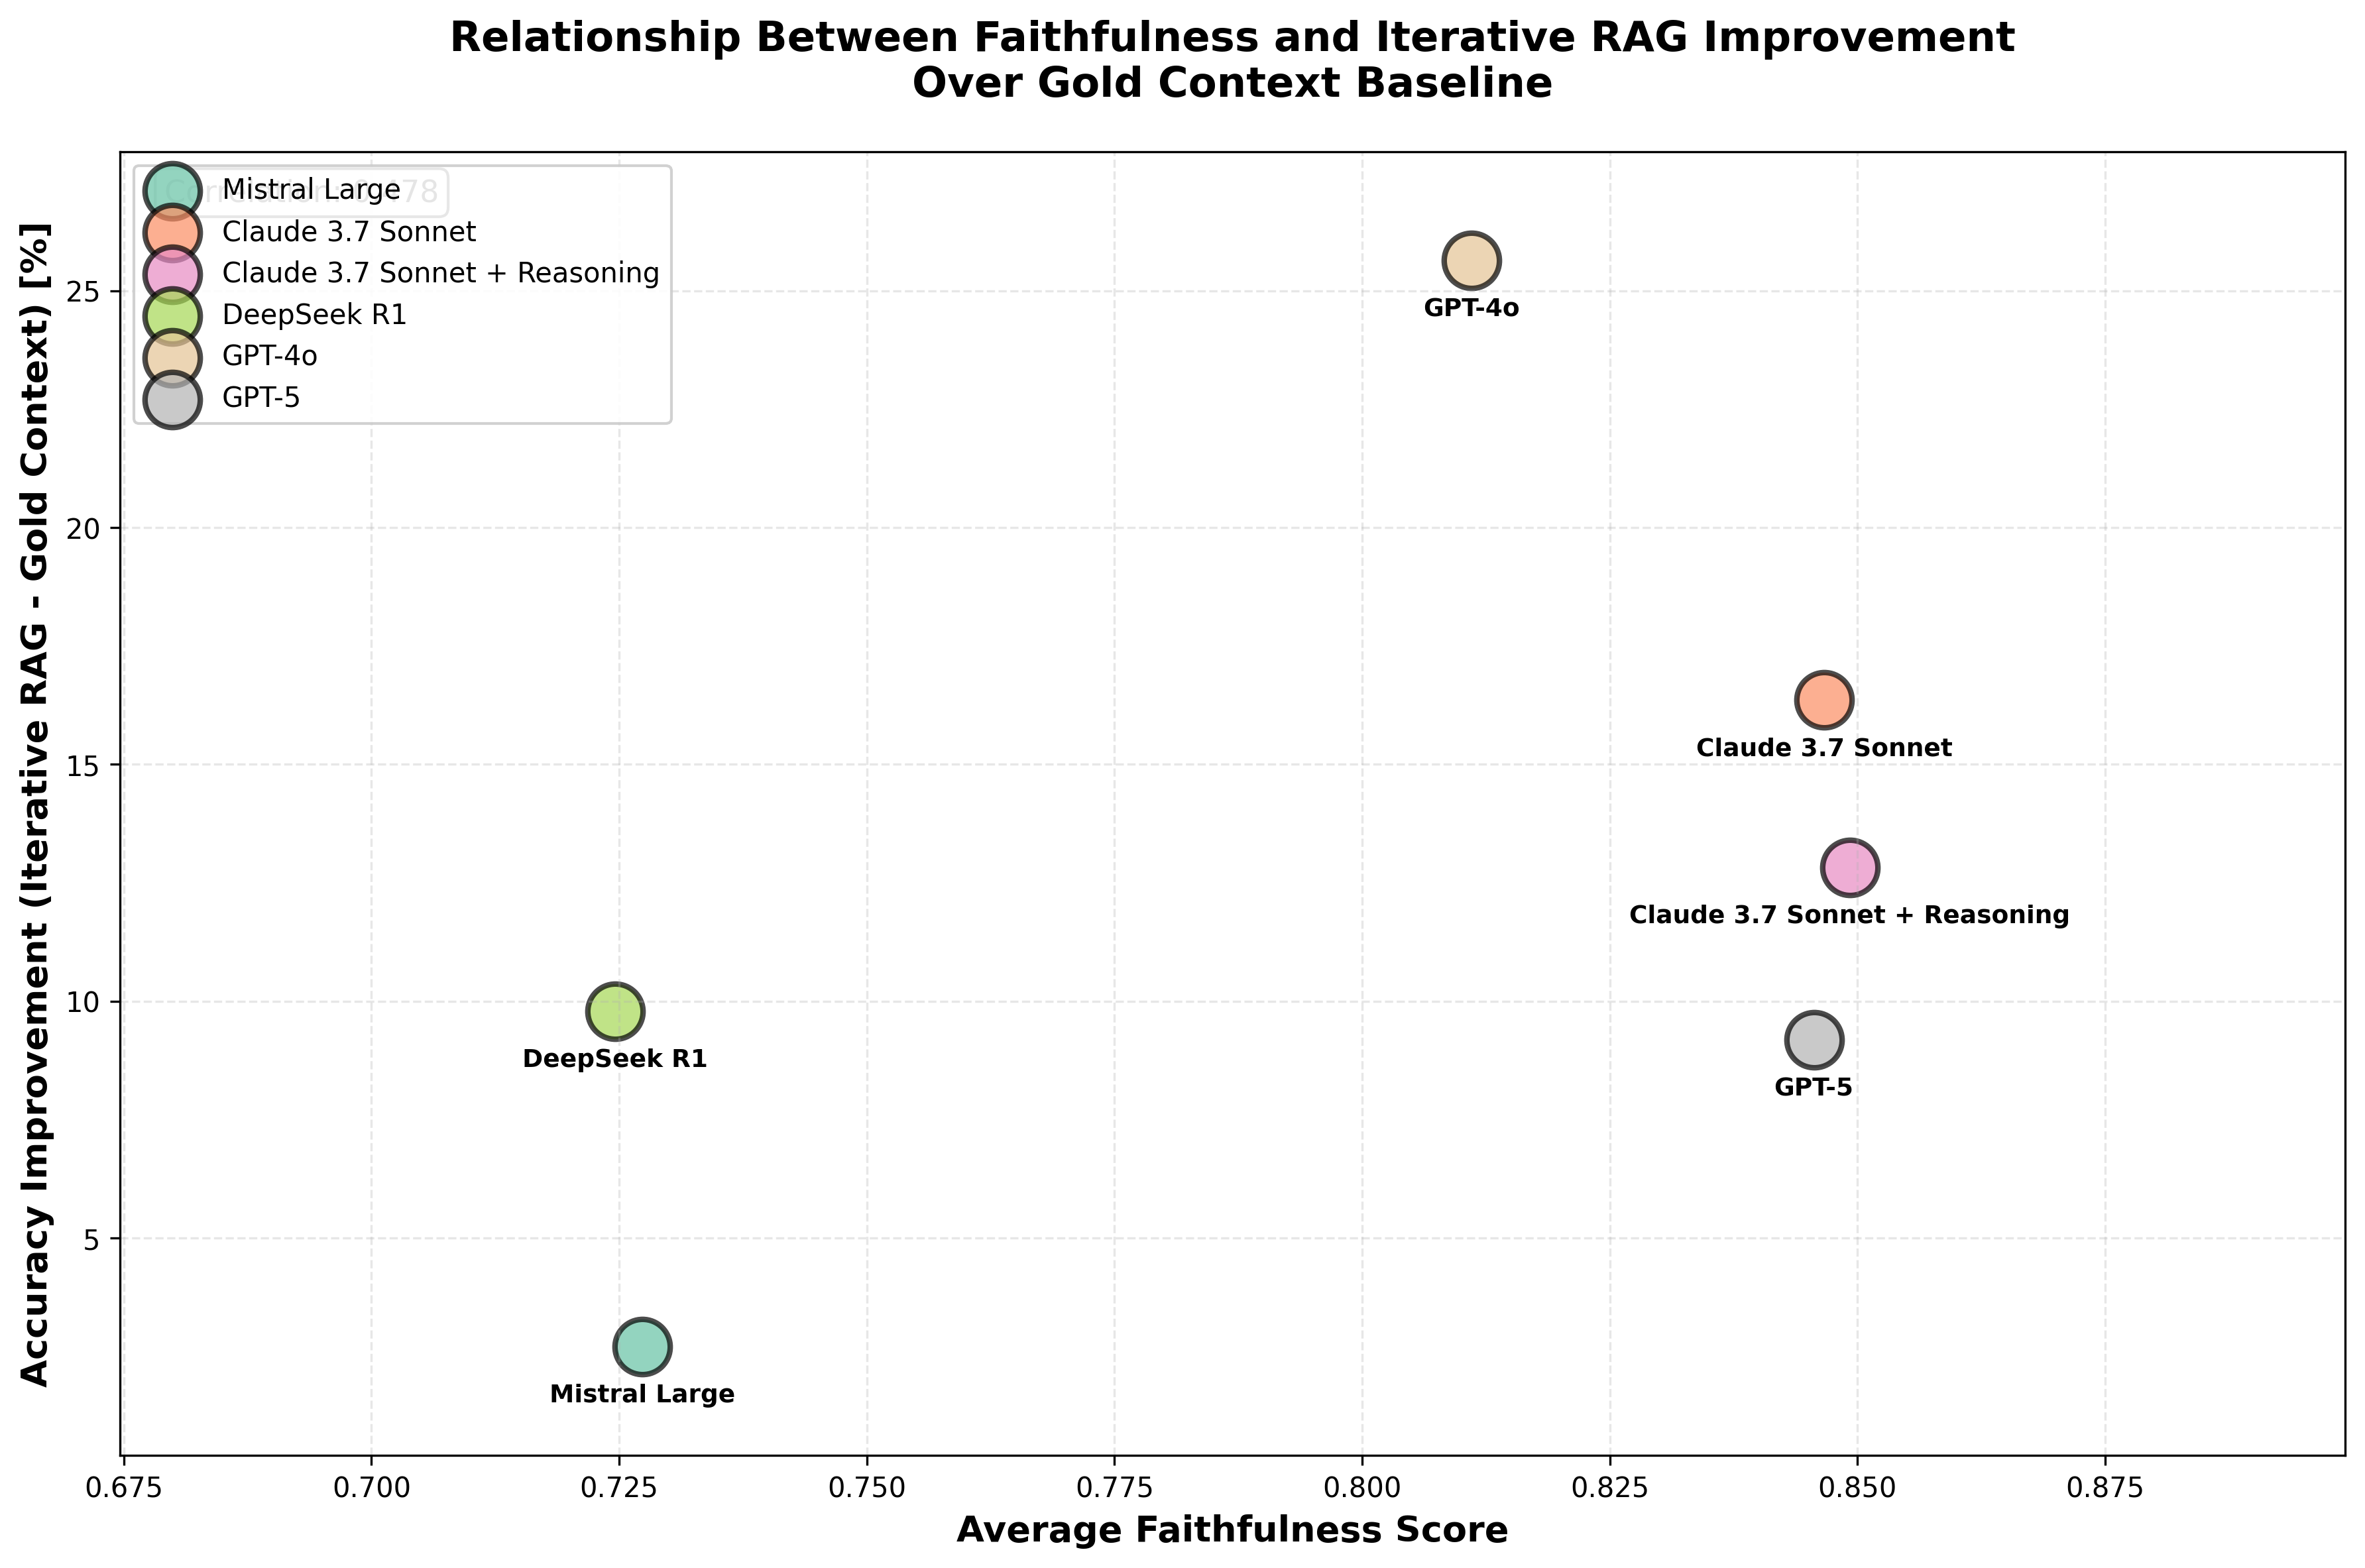
\includegraphics[width=0.7\linewidth]{src/chosen_plots/7_faithfulness_vs_improvement.png}
    \caption{Faithfulness vs. accuracy improvement. Iterative gains align with higher sufficiency and lower overconfidence.}
    \label{fig:faithfulness}
\end{figure}

\subsubsection{Sufficiency-Coverage Interaction}

The interaction between evidence sufficiency and retrieval coverage reveals a critical failure pattern (Figure~\ref{fig:sufficiency_coverage}):

\paragraph{Dangerous Quadrant:} Low coverage + Low sufficiency. This regime is most error-prone, characterized by both missing hops \emph{and} insufficient detail in retrieved documents.

\paragraph{Recoverable Scenarios:} High coverage with low sufficiency or low coverage with high sufficiency can sometimes still yield correct answers, but performance is most reliable in the high-coverage, high-sufficiency regime.

\textbf{Strategic Insight}: Systems should prioritize coverage first (retrieving documents for all hops), then sufficiency (retrieving detailed documents). The iterative loop is effective precisely because it can improve both dimensions over steps.

\begin{figure}[t]
    \centering
    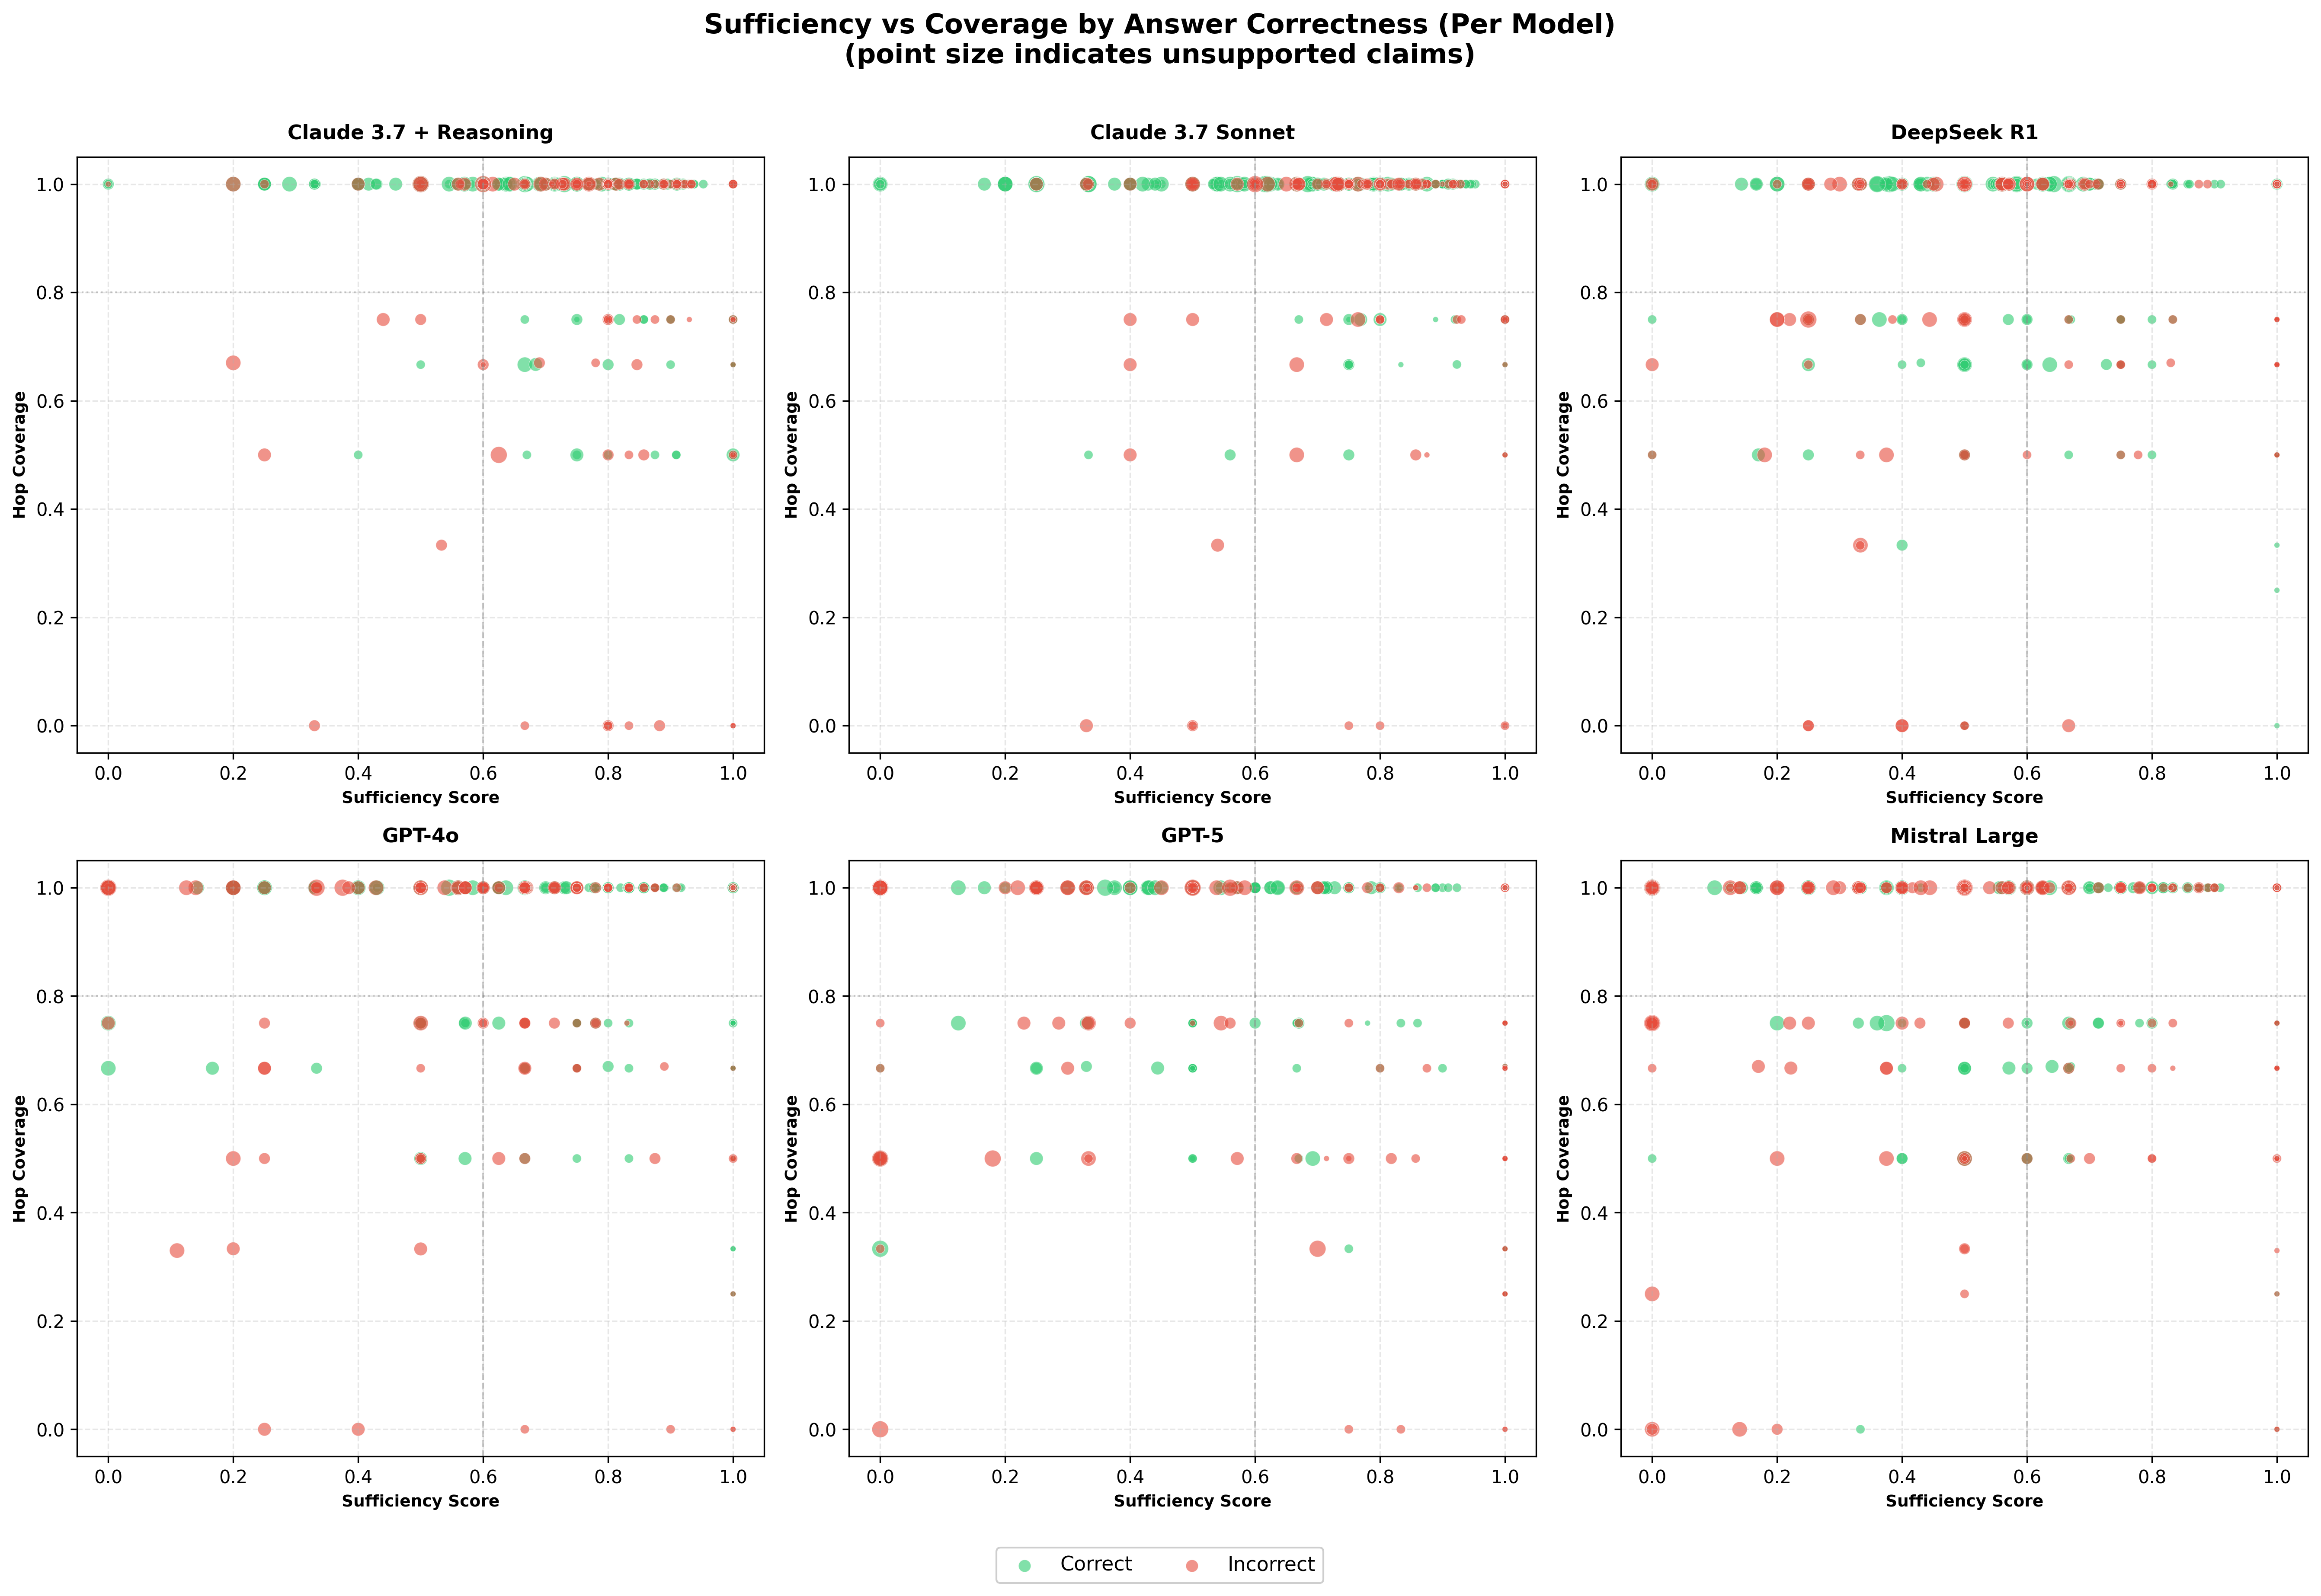
\includegraphics[width=0.8\linewidth]{src/chosen_plots/2_sufficiency_vs_coverage.png}
    \caption{Sufficiency-coverage interaction highlighting the "dangerous quadrant" (low coverage, low sufficiency). Coverage-first strategies, followed by sufficiency improvements, are most effective.}
    \label{fig:sufficiency_coverage}
\end{figure}

\subsection{Synthesis and Implications}

\subsubsection{Why Iterative RAG Outperforms Gold Context}

Our analysis suggests three mechanisms explain iterative RAG's superiority over gold context:

\paragraph{1. Cognitive Load Management:} Incremental information presentation reduces the ``needle in haystack'' problem. Models process 3--5 focused documents per step rather than 20--30 comprehensive documents simultaneously. Token usage analysis confirms that successful solutions use fewer, more targeted tokens.

\paragraph{2. Query Refinement:} Iterative approaches enable query reformulation based on partial answers. Successful multi-hop solutions frequently incorporate anchors and entities from earlier steps to refine subsequent queries.

\paragraph{3. Error Correction Opportunities:} Multiple retrieval cycles provide chances to recover from initial errors. Many ultimately correct answers involve backtracking or query reformulation, which is impossible in single-pass gold-context scenarios.

\subsubsection{Model Capability Spectrum}

Models fall along a capability spectrum for iterative RAG:

\paragraph{Tier 1 (GPT-5):} Robust across all question types, well-calibrated, minimal coverage gap impact, efficient token usage

\paragraph{Tier 2 (GPT-4o, DeepSeek R1):} Strong on moderate complexity, higher variance on hard questions, moderate calibration, sensitive to retrieval quality

\paragraph{Tier 3 (Claude variants, Mistral):} Struggle with complex composition, poor calibration, high coverage gap sensitivity, inconsistent reasoning patterns

Importantly, these tiers do NOT reflect overall model quality but specifically performance in iterative retrieval scenarios. The analysis suggests architectural features enabling robust iterative reasoning differ from those supporting strong zero-shot performance.

\subsubsection{Design Recommendations}

Based on failure mode analysis, we propose targeted improvements:

\paragraph{1. Coverage-First Retrieval:} Prioritize breadth (hitting all hops) over depth (comprehensive documents per hop). Implement hop-coverage estimation to trigger additional retrieval when gaps detected.

\paragraph{2. Early-Stage Verification:} Focus error detection and recovery on Hop 1--2, where failures cascade. Consider confidence-based re-retrieval for low-confidence initial steps.

\paragraph{3. Adaptive Stopping:} Implement stop criteria based on calibrated confidence rather than fixed step counts. Well-calibrated models achieve optimal accuracy 1--2 steps earlier than poorly calibrated models.

\paragraph{4. Sufficiency-Aware Selection:} Incorporate document sufficiency estimation into retrieval ranking. Prioritize documents with detailed technical content over broad overview documents.

\paragraph{5. Model-Specific Strategies:} Tailor retrieval strategies to model characteristics. High-variance models (DeepSeek R1) benefit from conservative, high-coverage retrieval; efficient models (GPT-5) benefit from aggressive early stopping.

\subsubsection{Limitations and Future Work}

Our analysis focuses on scientific multi-hop questions in chemistry. Generalization to other domains requires validation. Additionally, we identify several open questions:

\paragraph{1. Optimal Hop-Complexity Matching:} How should retrieval strategy adapt to estimated question complexity? Our analysis suggests current systems under-retrieve for complex questions and over-retrieve for simple ones.

\paragraph{2. Calibration Improvement:} Can we train models to better estimate confidence in iterative settings? The strong correlation between calibration and improvement suggests this is a high-leverage area.

\paragraph{3. Failure Prediction:} Can we predict coverage gaps or composition failures before final answer generation? Our sufficiency-coverage analysis suggests this may be possible.

\paragraph{4. Cross-Model Ensemble:} Given different model failure modes, can ensemble methods combine model strengths? GPT-5's robustness + DeepSeek R1's detailed reasoning + Claude's entity tracking could be complementary.

\subsection{Conclusion}

This analysis demonstrates that iterative RAG provides substantial advantages over gold context approaches, with performance improvements of \textbf{+2.7 to +25.6 percentage points} across diverse models (median ~+11.3 pp). Success stems from cognitive load management, query refinement capabilities, and error correction opportunities. However, models exhibit distinct behavioral patterns, with coverage gaps emerging as a primary failure mode that substantially reduces accuracy when present.

The observed relationship between calibration quality and iterative RAG benefit suggests that future improvements should focus on confidence estimation and adaptive retrieval strategies. Coverage-first retrieval, early-stage verification, and sufficiency-aware document selection emerge as high-priority system enhancements.

Most significantly, our analysis reveals that effective iterative RAG requires different model capabilities than zero-shot performance. The ability to integrate incremental information, maintain calibrated confidence, and recover from partial errors distinguishes high-performing models in iterative settings. These insights inform both retrieval system design and foundational model development for RAG applications.
